\documentclass[12pt,a4paper]{report}

% ==================== CẤU HÌNH CHUNG ====================
\usepackage{fontspec}
\setmainfont{Times New Roman}
\usepackage{amsmath,amsfonts,amssymb}
\usepackage{graphicx}
\usepackage{array,longtable,tabularx}
\usepackage{float}
\usepackage{caption}
\usepackage{geometry}
\usepackage{tikz}
\usetikzlibrary{arrows.meta,positioning,shapes.geometric}
\usepackage{titlesec}
\usepackage{enumitem}
\usepackage{setspace}
\usepackage{indentfirst}
\usepackage[table]{xcolor}
\usepackage{hyperref}
\usepackage{url}

\geometry{left=3cm,right=2cm,top=2.5cm,bottom=2.5cm}
\onehalfspacing
\setlength{\parindent}{1.27cm}
\setlength{\parskip}{3pt}
\setlist[itemize]{leftmargin=1.2cm,itemsep=2pt,topsep=3pt}
\setlist[enumerate]{leftmargin=1.2cm,itemsep=2pt,topsep=3pt}
\sloppy

\titleformat{\chapter}[block]{\normalfont\LARGE\bfseries\centering}{\thechapter.}{0.5em}{}
\titlespacing*{\chapter}{0pt}{-10pt}{20pt}
\setcounter{secnumdepth}{3}
\setcounter{tocdepth}{2}

\renewcommand{\contentsname}{MỤC LỤC}
\renewcommand{\listfigurename}{DANH MỤC HÌNH VẼ}
\renewcommand{\listtablename}{DANH MỤC BẢNG BIỂU}
\renewcommand{\bibname}{TÀI LIỆU THAM KHẢO}
\renewcommand{\figurename}{Hình}
\renewcommand{\tablename}{Bảng}

\hypersetup{
    colorlinks=true,
    linkcolor=black,
    citecolor=black,
    urlcolor=blue,
    pdftitle={Hệ thống phân tích tín hiệu khuếch đại},
    pdfauthor={Nguyễn Duy Anh; Nguyễn Văn Dương}
}

\newcommand{\code}[1]{\texttt{#1}}
\newcommand{\unit}[1]{\,\mathrm{#1}}
\newcommand{\NA}{\textit{Không áp dụng}}
\newcommand{\tableheadcolor}{\rowcolor{gray!18}}
\setlength{\arrayrulewidth}{0.6pt}
\renewcommand{\arraystretch}{1.2}
\newcolumntype{Y}{>{\raggedleft\arraybackslash}X}

\begin{document}

% ==================== TRANG BÌA ====================
\begin{titlepage}
    \begin{tikzpicture}[remember picture,overlay]
        \draw[line width=1.5pt]
            ([xshift=3cm,yshift=-2.5cm]current page.north west)
            rectangle
            ([xshift=-2cm,yshift=2.5cm]current page.south east);
    \end{tikzpicture}

    \begin{center}
        \vspace*{0.5cm}
        \large \textbf{ĐẠI HỌC BÁCH KHOA HÀ NỘI}\\
        \large \textbf{TRƯỜNG ĐIỆN -- ĐIỆN TỬ}

        \vspace{2.2cm}
        \Huge \textbf{BÁO CÁO}

        \vspace{1.5cm}
        \large \textbf{ĐỒ ÁN CHUYÊN NGÀNH II}

        \vspace{1cm}
        {\Large \textbf{NGHIÊN CỨU, THIẾT KẾ VÀ CHẾ TẠO\\[0.2cm]
        HỆ THỐNG PHÂN TÍCH TÍN HIỆU KHUẾCH ĐẠI}}

        \vspace{2.2cm}
        \begin{table}[h]
            \centering
            \large
            \renewcommand{\arraystretch}{1.3}
            \begin{tabular}{ll}
                \textbf{Sinh viên thực hiện:} & Nguyễn Duy Anh -- 20241652E \\
                                               & Nguyễn Văn Dương -- 20241713E \\[0.5cm]
                \textbf{GVHD:} & TS. Đào Việt Hùng
            \end{tabular}
        \end{table}

        \vfill
        \large Hà Nội, 7--2026
        \vspace*{0.5cm}
    \end{center}
\end{titlepage}

% ==================== PHẦN ĐẦU ====================
\pagenumbering{roman}

\chapter*{LỜI CẢM ƠN}
\addcontentsline{toc}{chapter}{LỜI CẢM ƠN}
Nhóm sinh viên xin trân trọng cảm ơn TS. Đào Việt Hùng đã định hướng, góp ý chuyên môn và hỗ trợ nhóm trong suốt quá trình thực hiện đồ án. Những trao đổi về kiến trúc hệ thống đo, thiết kế phần cứng tương tự, lập trình nhúng và phương pháp trình bày kết quả đã giúp nhóm hoàn thiện sản phẩm theo hướng có khả năng kiểm chứng và mở rộng. Nhóm cũng xin cảm ơn các thầy cô Trường Điện -- Điện tử, Đại học Bách khoa Hà Nội đã cung cấp nền tảng kiến thức cần thiết về điện tử, vi điều khiển và xử lý tín hiệu số.

Do phạm vi đề tài bao gồm cả phần cứng, firmware và phần mềm máy tính, báo cáo khó tránh khỏi những thiếu sót. Nhóm mong nhận được các ý kiến phản biện để tiếp tục hoàn thiện độ chính xác đo lường và khả năng ứng dụng của hệ thống.
\clearpage

\chapter*{TÓM TẮT ĐỒ ÁN}
\addcontentsline{toc}{chapter}{TÓM TẮT ĐỒ ÁN}
Đồ án trình bày quá trình nghiên cứu và xây dựng nguyên mẫu hệ thống phân tích tín hiệu khuếch đại có khả năng phát tín hiệu thử, thu đồng thời điện áp vào và điện áp ra của thiết bị cần đo, truyền dữ liệu về máy tính và đánh giá chất lượng phép đo. Hệ thống sử dụng vi điều khiển STM32F103C8T6 làm bộ điều khiển trung tâm, DAC kép MCP4822 để tạo tín hiệu kích thích, ADC lấy mẫu đồng thời ADS7861 để thu hai kênh và USB CDC Full Speed để giao tiếp với máy tính.

Firmware được xây dựng trên STM32 HAL và PlatformIO, bao gồm driver SPI--DMA cho DAC/ADC, điều khiển ba dải đo, hiệu chuẩn lưu trong Flash, bộ phân tích lệnh ASCII và giao thức truyền mẫu nhị phân có kiểm tra XOR. Ứng dụng Signal Analyzer Pro sử dụng Python, PyQt6, PyQtGraph, NumPy, SciPy và PySerial. Phần mềm cung cấp waveform, quét Bode, phân tích từng kênh, tính gain/phase/delay, đánh giá điều kiện lấy mẫu, phát hiện clipping/saturation và kết luận PASS/FAIL/WARNING. Luồng đọc USB chạy trên tiến trình riêng nhằm tránh khóa giao diện.

Kết quả kiểm nghiệm gần nhất xác nhận chuỗi đo phần cứng thật từ DAC qua DUT/AFE tới ADS7861 và ứng dụng desktop. ADC hoạt động liên tục theo timer--SPI--DMA ở tốc độ thực tế $140{,}077\unit{SPS}$; DAC sử dụng DMA với nhịp cập nhật độc lập. Chín cấu hình thực nghiệm đã được chụp trực tiếp trên ứng dụng, gồm quét $100\unit{Hz}$ đến $20\unit{kHz}$ và thay đổi biên độ/dải đo. Dạng sóng tần số thấp thể hiện tốt, trong khi $20\unit{kHz}$ chỉ còn khoảng 7 mẫu mỗi chu kỳ. Các ca tín hiệu nhỏ, clipping và bão hòa ADC cũng cho thấy giới hạn của AFE, lựa chọn range và thuật toán khi tỷ số tín hiệu trên nhiễu thấp. Vì vậy hệ thống đã vượt qua giai đoạn bring-up giao tiếp, nhưng vẫn cần hiệu chuẩn và tối ưu để trở thành thiết bị đo định lượng có độ chính xác cao.

\textbf{Từ khóa:} STM32F103, MCP4822, ADS7861, USB CDC, signal analyzer, gain, phase, Bode, sine fitting.
\clearpage

\tableofcontents
\clearpage
\listoffigures
\clearpage
\listoftables
\clearpage

\chapter*{DANH MỤC TỪ VIẾT TẮT}
\addcontentsline{toc}{chapter}{DANH MỤC TỪ VIẾT TẮT}
\begin{longtable}{|p{2.3cm}|p{4.7cm}|p{5.8cm}|}
\hline
\tableheadcolor\textbf{Viết tắt} & \textbf{Dạng đầy đủ} & \textbf{Giải nghĩa} \\ \hline
\endfirsthead
\hline
\tableheadcolor\textbf{Viết tắt} & \textbf{Dạng đầy đủ} & \textbf{Giải nghĩa} \\ \hline
\endhead
ADC & Analog-to-Digital Converter & Bộ chuyển đổi tương tự sang số \\ \hline
AFE & Analog Front-End & Mạch điều hòa tín hiệu tương tự \\ \hline
CDC & Communications Device Class & Lớp thiết bị truyền thông USB \\ \hline
DAC & Digital-to-Analog Converter & Bộ chuyển đổi số sang tương tự \\ \hline
DSP & Digital Signal Processing & Xử lý tín hiệu số \\ \hline
DUT & Device Under Test & Mạch hoặc thiết bị cần đo \\ \hline
FFT & Fast Fourier Transform & Biến đổi Fourier nhanh \\ \hline
FS & Full Speed & Chế độ USB tốc độ 12 Mbit/s \\ \hline
GUI & Graphical User Interface & Giao diện người dùng đồ họa \\ \hline
MCU & Microcontroller Unit & Vi điều khiển \\ \hline
PMA & Packet Memory Area & Vùng nhớ gói tin USB của STM32F1 \\ \hline
RMS & Root Mean Square & Giá trị hiệu dụng \\ \hline
SPI & Serial Peripheral Interface & Giao tiếp ngoại vi nối tiếp \\ \hline
SWD & Serial Wire Debug & Giao diện nạp và gỡ lỗi \\ \hline
THD & Total Harmonic Distortion & Tổng méo hài \\ \hline
USB & Universal Serial Bus & Chuẩn kết nối nối tiếp đa dụng \\ \hline
ZOH & Zero-Order Hold & Cơ chế giữ mẫu bậc không \\ \hline
\end{longtable}
\clearpage

% ==================== NỘI DUNG ====================
\pagenumbering{arabic}

\chapter{MỞ ĐẦU}

\section{Lý do lựa chọn đề tài}
Đáp ứng biên độ và pha là hai đặc trưng cơ bản quyết định khả năng làm việc của một mạch khuếch đại. Trong quá trình học tập, thiết kế và sửa chữa mạch điện tử, người thực hiện thường cần đồng thời một nguồn phát tín hiệu, một dao động ký và công cụ xử lý số để xác định hệ số khuếch đại, độ lệch pha và băng thông. Các thiết bị thương mại đáp ứng tốt yêu cầu này nhưng chi phí tương đối cao, trong khi các giải pháp dựa trên vi điều khiển thường chỉ dừng ở hiển thị waveform và chưa đánh giá độ tin cậy của điều kiện đo.

Từ nhu cầu đó, nhóm lựa chọn xây dựng một hệ thống tích hợp gồm phần cứng phát/thu, firmware điều khiển và ứng dụng máy tính. Ngoài việc hiển thị tín hiệu, hệ thống phải chỉ ra khi nào kết quả có thể tin cậy. Ví dụ, ở cấu hình mục tiêu $20\unit{kHz}/200\unit{kSPS}$, mỗi chu kỳ chỉ có 10 điểm; nếu chỉ dùng cực đại/cực tiểu, sai số bắt hụt đỉnh có thể gần $4{,}9\%$. Mặt khác, chu kỳ cập nhật DAC là $5\unit{\mu s}$, chỉ lớn hơn thời gian xác lập điển hình của MCP4822 khoảng $0{,}5\unit{\mu s}$. Đây là phân tích cấu hình mục tiêu; ADC hiện chưa đạt tốc độ pacing này. Vì vậy, một nhãn PASS không kèm trạng thái xác minh timing sẽ tạo cảm giác chính xác giả tạo.

\section{Mục tiêu của đề tài}
Mục tiêu tổng quát là chế tạo một hệ thống phân tích tín hiệu khuếch đại có khả năng hoạt động độc lập với thiết bị đo chuyên dụng trong các bài thử cơ bản. Các mục tiêu cụ thể gồm:
\begin{itemize}
    \item Phát tín hiệu sine, square, triangle và DC với tần số, biên độ, offset và bit gain cấu hình được.
    \item Thu đồng thời hai kênh $V_{in}$ và $V_{out}$ bằng ADC 12-bit, hỗ trợ ba dải đo $0{,}3\unit{V}$, $3{,}3\unit{V}$ và $10\unit{V}$.
    \item Truyền lệnh và dữ liệu qua USB CDC, có cơ chế kiểm tra độ dài và tính toàn vẹn của frame.
    \item Đo Vmax, Vmin, Vpp, RMS AC, offset, tần số, gain, phase, delay, noise residual, clipping và saturation.
    \item Đánh giá điều kiện lấy mẫu, sai số DAC và đưa ra PASS/FAIL/WARNING rõ ràng.
    \item Cho phép chạy simulation khi không có phần cứng, quản lý calibration và xuất báo cáo CSV/JSON.
\end{itemize}

\section{Đối tượng và phạm vi nghiên cứu}
Đối tượng nghiên cứu là các mạch khuếch đại điện áp làm việc với tín hiệu tuần hoàn trong dải thấp và trung bình, ưu tiên tín hiệu sine quanh $20\unit{kHz}$. Hệ thống tập trung vào phép đo hai kênh, đặc tuyến gain/phase và đáp ứng tần số. Các phép đo chuyên sâu như trở kháng vào/ra, CMRR, PSRR, THD+N chuẩn phòng thí nghiệm và công suất tải lớn nằm ngoài phạm vi chính.

Phần cứng trung tâm là STM32F103C8T6, DAC MCP4822 và ADC ADS7861. Phần mềm desktop chạy trên Windows bằng Python/PyQt6. Báo cáo phân biệt ba lớp bằng chứng: kết quả simulation/DSP, phép thử USB trên bo mạch thật và phép đo analog end-to-end. Cả ba lớp đã được kiểm nghiệm; riêng phép đo analog vẫn cần hiệu chuẩn định lượng và đánh giá độ không đảm bảo đo.

\section{Phương pháp thực hiện}
Đề tài được triển khai theo hướng chia hệ thống thành các lớp có thể kiểm thử độc lập. Phần cứng được phân thành chuỗi TX, DUT và chuỗi RX. Firmware được tách thành driver thiết bị, bộ điều khiển phép đo, giao thức và USB. Ứng dụng desktop tách phần giao diện, worker truyền thông và module phân tích tín hiệu. Mỗi lớp được kiểm tra trước khi ghép nối toàn hệ thống.

Các công thức sai số được kiểm thử bằng unit test. Giao thức USB được thử bằng lệnh request/response, kiểm tra frame nhị phân và checksum. Kết quả đo được so sánh với tham số cấu hình chuẩn của bộ mô phỏng và DUT tham chiếu.

\section{Bố cục báo cáo}
Báo cáo gồm bảy chương. Chương 1 trình bày bài toán và mục tiêu. Chương 2 tổng hợp cơ sở lý thuyết. Chương 3 mô tả thiết kế hệ thống và phần cứng. Chương 4 trình bày firmware và giao thức. Chương 5 trình bày ứng dụng desktop và DSP. Chương 6 mô tả kiểm nghiệm, kết quả và thảo luận. Chương 7 tổng kết và đề xuất hướng phát triển.

\chapter{TỔNG QUAN VÀ CƠ SỞ LÝ THUYẾT}

\section{Tổng quan thiết bị phân tích mạch khuếch đại}
Một bộ phân tích mạch khuếch đại cần tạo tín hiệu kích thích có tham số biết trước, đo đồng thời tín hiệu trước và sau DUT, sau đó suy ra các đặc tính truyền đạt. Khác với dao động ký chỉ hiển thị dạng sóng, bộ phân tích phải gắn kết kết quả với điều kiện đo, độ chính xác và tiêu chí nghiệm thu. Kiến trúc phổ biến gồm nguồn phát, AFE, ADC hai kênh, bộ xử lý và giao diện hiển thị.

Giải pháp của đề tài sử dụng các linh kiện rời thay vì DAC/ADC nội của MCU. MCP4822 cung cấp hai kênh DAC 12-bit, tham chiếu nội và bit gain; ADS7861 cung cấp hai ADC 12-bit lấy mẫu đồng thời, phù hợp với phép đo pha vì giảm sai lệch thời điểm giữa hai kênh \cite{mcp4822,ads7861}. STM32F103 đảm nhiệm điều phối thời gian, SPI, USB và quản lý cấu hình \cite{stm32ds,stm32rm}.

\section{Các thông số đánh giá bộ khuếch đại}
Với hai chuỗi điện áp $v_{in}[n]$ và $v_{out}[n]$, giá trị trung bình và RMS thành phần AC được xác định bởi:
\begin{align}
\overline{v} &= \frac{1}{M}\sum_{n=0}^{M-1}v[n],\\
V_{\mathrm{RMS,AC}} &= \sqrt{\frac{1}{M}\sum_{n=0}^{M-1}\left(v[n]-\overline{v}\right)^2}.
\end{align}
Sử dụng RMS AC giúp loại ảnh hưởng của offset DC và ít nhạy với việc bỏ lỡ đúng đỉnh hơn Vpp. Hệ số khuếch đại được tính theo:
\begin{align}
G_{lin} &= \frac{V_{out,\mathrm{RMS,AC}}}{V_{in,\mathrm{RMS,AC}}},\\
G_{dB} &= 20\log_{10}(G_{lin}).
\end{align}

Để xác định phase, ứng dụng khớp tín hiệu với mô hình:
\begin{equation}
v(t)=A\sin(2\pi ft+\phi)+C+e(t),
\end{equation}
trong đó $A$ là biên độ, $C$ là offset và $e(t)$ là phần dư. Hiệu phase giữa hai kênh là $\Delta\phi=\phi_{out}-\phi_{in}$, được chuẩn hóa vào khoảng $[-180^\circ,180^\circ]$. Độ trễ tương đương:
\begin{equation}
\tau=\frac{\Delta\phi}{360^\circ f}.
\end{equation}

\section{Cơ sở lý thuyết lấy mẫu tín hiệu}
Điều kiện Nyquist yêu cầu $F_s>2f_{max}$ để tránh chồng phổ \cite{oppenheim}. Tuy nhiên, thỏa mãn Nyquist chưa đồng nghĩa waveform có đủ điểm để đo peak và phase chính xác. Số mẫu trên mỗi chu kỳ là:
\begin{equation}
N=\frac{F_s}{f_{signal}}.
\end{equation}
Chu kỳ tín hiệu và khoảng thời gian giữa hai mẫu:
\begin{equation}
T_{signal}=\frac{10^6}{f_{signal}}\;[\mu s],\qquad
T_s=\frac{10^6}{F_s}\;[\mu s].
\end{equation}

Trong trường hợp xấu nhất, điểm lấy mẫu gần đỉnh sine bị lệch nửa bước pha. Sai số peak lý thuyết được ước lượng:
\begin{equation}
E_{peak}=\left(1-\cos\frac{\pi}{N}\right)\times100\%.
\end{equation}
Đây là lý do ứng dụng ưu tiên RMS AC và sine fit, đồng thời vẫn hiển thị Vmax/Vmin để người dùng quan sát trực tiếp.

\section{Đặc tính và sai số của ADC, DAC}
DAC dạng bậc thang tương đương một bộ giữ mẫu bậc không. Suy hao biên độ chuẩn hóa tại tần số tín hiệu được xấp xỉ:
\begin{equation}
E_{ZOH}=\left(1-\frac{\sin(\pi/N)}{\pi/N}\right)\times100\%.
\end{equation}
MCP4822 có độ phân giải 12-bit và thời gian xác lập điển hình khoảng $4{,}5\unit{\mu s}$ \cite{mcp4822}. Biên thời gian xác lập được định nghĩa:
\begin{equation}
T_{margin}=T_s-T_{settling}.
\end{equation}
Nếu $T_{margin}<0$, mẫu DAC mới được cập nhật trước khi đầu ra ổn định; nếu $0\leq T_{margin}<1\unit{\mu s}$, phép phát được đánh giá borderline.

Với ADC 12-bit, mã số nằm trong khoảng 0--4095. Sau khi trừ mức bias $1{,}65\unit{V}$ và áp dụng calibration cho từng dải đo, điện áp đầu vào được tính:
\begin{equation}
V_{in}=m_r\left(\frac{code}{4095}\cdot3{,}3-1{,}65\right)+c_r,
\end{equation}
trong đó $m_r$ và $c_r$ là hệ số scale/offset của range $r$. Các mã gần 0 hoặc 4095 được đánh dấu saturation.

\section{Phương pháp đánh giá kết quả}
Kết quả tổng thể không chỉ dựa trên gain. Hệ thống phân biệt ba trạng thái:
\begin{itemize}
    \item \textbf{PASS}: gain, tần số, biên độ đạt tolerance; không clipping/saturation; frame đầy đủ; điều kiện đo hợp lệ.
    \item \textbf{FAIL}: ít nhất một yêu cầu kỹ thuật không đạt hoặc có lỗi truyền thông/mất dữ liệu.
    \item \textbf{WARNING}: tín hiệu có thể đạt yêu cầu nhưng độ tin cậy bị giới hạn bởi số mẫu/chu kỳ, sai số peak hoặc biên xác lập DAC.
\end{itemize}
Quy tắc này ngăn trường hợp $N=10$ bị hiển thị PASS xanh tuyệt đối dù sai số peak lý thuyết gần $4{,}9\%$.

\chapter{THIẾT KẾ HỆ THỐNG}

\section{Yêu cầu kỹ thuật}
Các yêu cầu chính của nguyên mẫu được tổng hợp trong Bảng \ref{tab:requirements}.
\begin{table}[H]
\centering
\caption{Yêu cầu kỹ thuật chính của hệ thống}
\label{tab:requirements}
\begin{tabularx}{\textwidth}{|p{4.2cm}|X|}
\hline
\tableheadcolor\textbf{Hạng mục} & \textbf{Yêu cầu} \\ \hline
Bộ xử lý & STM32F103C8T6, xung nhịp hệ thống $72\unit{MHz}$ \\ \hline
Khối phát & DAC MCP4822 12-bit, SPI, gain X1/X2 \\ \hline
Khối thu & ADS7861 12-bit, hai kênh lấy mẫu đồng thời \\ \hline
Dải đo & Auto hoặc manual: $0{,}3\unit{V}$, $3{,}3\unit{V}$, $10\unit{V}$ \\ \hline
Giao tiếp & USB CDC FS, cổng COM ảo trên Windows \\ \hline
Độ dài capture & 128, 256 hoặc 512 cặp mẫu; firmware chặn cấu hình lớn hơn 512 \\ \hline
Chế độ đo & Single tone, waveform, passive oscilloscope, Bode sweep \\ \hline
Kết quả & Channel metrics, DUT metrics và PASS/FAIL/WARNING \\ \hline
Vận hành không thiết bị & Có chế độ simulation/mock \\ \hline
\end{tabularx}
\end{table}

\section{Kiến trúc tổng thể}
Hình \ref{fig:system_arch} là sơ đồ khối chức năng được sử dụng trong quá trình triển khai PCB. Máy tính gửi cấu hình qua USB CDC; STM32 điều khiển DAC tạo tín hiệu kích thích cho DUT; nhánh trên hồi tiếp tín hiệu phát để quan sát $V_{in}$ và nhánh dưới nhận $V_{out}$ qua bộ chọn dải. Hai khối ADC1/ADC2 trong hình biểu diễn hai lõi chuyển đổi đồng thời A/B bên trong ADS7861, không phải hai IC ADC độc lập. Dữ liệu hai kênh được STM32 truyền lại cho ứng dụng desktop để hiển thị và phân tích.

\begin{figure}[H]
\centering

\includegraphics[width=\textwidth]{\detokenize{images/Sơ đồ khối/image.png}}
\caption{Kiến trúc tổng thể của hệ thống theo sơ đồ khối thiết kế}
\label{fig:system_arch}
\end{figure}

\section{Thiết kế khối phát tín hiệu}
MCP4822 là DAC hai kênh 12-bit, giao tiếp SPI và có tham chiếu nội $2{,}048\unit{V}$. Word điều khiển 16-bit gồm bit chọn kênh, bit gain, bit shutdown và 12 bit dữ liệu \cite{mcp4822}. STM32 sử dụng SPI1; chân PA4 làm chip-select phần mềm và PA3 nối với LDAC. Firmware giữ LDAC ở mức thấp để đầu ra được cập nhật sau khi hoàn tất mỗi frame SPI. Driver đóng gói dữ liệu big-endian và giữ CS ở mức thấp trong toàn bộ hai byte truyền.

Firmware tạo bảng mẫu theo dạng sóng, tần số, biên độ và offset. Do MCP4822 là DAC đơn cực, firmware cộng mức bias $1{,}65\unit{V}$ trước khi mã hóa; tầng analog TX trừ lại mức này để thu được tín hiệu lưỡng cực quanh $0\unit{V}$. Hệ số hiệu chuẩn DAC X2 được mô tả bằng quan hệ tuyến tính $V=a\cdot code+b$; với X1, scale mV/code bằng một nửa X2. Mã phát được giới hạn trong khoảng 0--4095.
\begin{equation}
code=\mathrm{clip}\left(\frac{V_{signal}+V_{bias}-b}{a\,s_G},0,4095\right),
\qquad s_G=\begin{cases}1,&G=\mathrm{X2}\\0{,}5,&G=\mathrm{X1}.\end{cases}
\end{equation}
Đầu ra DAC được đưa qua buffer/lọc tái tạo trước khi cấp cho DUT. Khi lựa chọn tốc độ cập nhật, ứng dụng đồng thời tính ZOH droop và settling margin để cảnh báo người vận hành.

Số điểm của LUT được firmware tính bằng phép chia nguyên $N=F_s/f$ và giới hạn trong khoảng 10--256. Vì vậy tần số phát thực là $f_{DAC}=F_{update}/N$ và chỉ trùng tần số yêu cầu khi tỷ số $F_s/f$ phù hợp với giới hạn LUT. Với cấu hình mặc định $20\unit{kHz}/200\unit{kSPS}$, $N=10$ và DAC stream phát đúng $20\unit{kHz}$. Ngược lại, nếu yêu cầu $30\unit{kHz}$ tại $200\unit{kSPS}$ thì $N$ tính được bằng 6 nhưng bị ép thành 10, dẫn tới tần số phát thực khoảng $20\unit{kHz}$.

Luồng hiện tại dùng timer và DMA để tách nhịp phát DAC khỏi công việc giao thức USB. TIM3 nhận clock $72\unit{MHz}$; ở cấu hình $ARR=359$, tốc độ cập nhật đạt $200\unit{kSPS}$. SPI1 chạy $18\unit{MHz}$ nên một frame DAC 16-bit cần khoảng $0{,}89\unit{\mu s}$ trên đường truyền, chưa kể thời gian chốt dữ liệu. Chu kỳ cập nhật $5\unit{\mu s}$ chỉ lớn hơn settling time điển hình $4{,}5\unit{\mu s}$ một biên nhỏ; đây là giới hạn analog của MCP4822 dù DMA đã giảm đáng kể tải CPU.

\section{Thiết kế khối thu tín hiệu hai kênh}
ADS7861 tích hợp hai ADC 12-bit và hỗ trợ lấy mẫu đồng thời, tốc độ tới $500\unit{kSPS}$ theo datasheet \cite{ads7861}. Thiết kế sử dụng Mode II: M0=0, M1=1; kết quả A và B được đọc tuần tự trên đường Serial Data A. PA8 tạo xung RD/CONVST, PB10 nối BUSY và PB12 điều khiển CS. Mỗi cặp kết quả cần 32 clock trên Serial Data A; firmware tách status và dữ liệu signed 12-bit rồi chuyển sang offset-binary trước khi đưa vào pipeline USB hiện có.

Trong cấu hình production, timer tạo nhịp chuyển đổi đều và SPI2--DMA thu các word của ADS7861 vào buffer liên tục. ISR chỉ xử lý sự kiện ngắn và phần ghép frame, chuyển đổi mã, truyền USB được đẩy ra luồng nền. Đợt kiểm nghiệm thực tế đạt $140{,}077\unit{SPS}$ cho mỗi cặp hai kênh. Cách tổ chức này loại bỏ giới hạn của driver GPIO bit-bang ban đầu, nhưng vẫn phải theo dõi cờ overrun và sequence của buffer khi tiếp tục tăng tốc độ.

Hai kênh được ghép vào một word 32-bit: CH1 ở 16 bit cao, CH2 ở 16 bit thấp. Buffer production hiện có tối đa 512 cặp mẫu, chiếm $2048\unit{byte}$. Việc giảm buffer là cần thiết để giữ biên SRAM an toàn trên STM32F103 có $20\unit{kB}$ SRAM.

\section{Mạch điều hòa và lựa chọn range}
Tín hiệu lưỡng cực được bias quanh $1{,}65\unit{V}$ để phù hợp với dải ADC đơn cực. Ba nhánh range tương ứng mức trực tiếp, suy hao xấp xỉ 10 lần và 100 lần. Các relay được đóng theo cơ chế break-before-make để không kích hoạt đồng thời hai nhánh. Hệ thống khởi động ở dải $10\unit{V}$ nhằm bảo vệ ADC trước một tín hiệu chưa biết.

Trong chế độ AUTO, firmware xác định khoảng cách lớn nhất từ mã giữa 2048 và đếm số mẫu gần rail. Nếu xuất hiện rail hit, range được tăng; nếu biên độ quá nhỏ, range được giảm. Sau khi chuyển relay, dữ liệu được thu lại để đảm bảo kết quả dùng đúng hệ số calibration.

\section{Nguồn, kết nối và phân bổ chân}
STM32 sử dụng nguồn $3{,}3\unit{V}$, thạch anh ngoài $8\unit{MHz}$ và PLL để đạt $72\unit{MHz}$. Các tụ decoupling được đặt gần chân nguồn số, nguồn tương tự và nguồn tham chiếu. Đường USB D-/D+ nối PA11/PA12, có trở kháng vi sai và chiều dài tương đối cân bằng. SWD trên PA13/PA14 được giữ lại để nạp và debug; chỉ JTAG bị vô hiệu hóa khi cần giải phóng chân.

\begin{table}[H]
\centering
\caption{Phân bổ các chân điều khiển chính}
\label{tab:pinmap}
\begin{tabularx}{\textwidth}{|p{3cm}|p{3.8cm}|X|}
\hline
\tableheadcolor\textbf{Khối} & \textbf{Chân STM32} & \textbf{Chức năng} \\ \hline
MCP4822 & PA3, PA4, PA5, PA7 & LDAC, CS, SPI1 SCK, SPI1 MOSI \\ \hline
ADS7861 & PB13, PB14 & CLOCK GPIO bring-up, Serial Data A \\ \hline
ADS7861 & PA8, PB10, PB12 & RD/CONVST, BUSY, CS \\ \hline
ADS7861 & PB0, PB1, PB11 & M0, A0, M1 \\ \hline
Range & PA15, PB3, PB4 & Relay $0{,}3\unit{V}$, $3{,}3\unit{V}$, $10\unit{V}$ \\ \hline
USB FS & PA11, PA12 & D-, D+ \\ \hline
Debug & PA13, PA14 & SWDIO, SWCLK \\ \hline
\end{tabularx}
\end{table}

\section{PCB và nguyên mẫu phần cứng}
Hình \ref{fig:pcb_3d} và Hình \ref{fig:pcb_layout} trình bày mô hình bố trí linh kiện, lớp đồng và các vùng analog/digital của PCB. Ba relay công suất nằm ở phía phải; STM32, cổng USB và header debug nằm ở phía trái. Các nhãn Analog/Digital trên silkscreen hỗ trợ kiểm tra phân vùng khi lắp ráp và debug.

\begin{figure}[H]
\centering
\begin{minipage}[t]{0.49\textwidth}
\centering
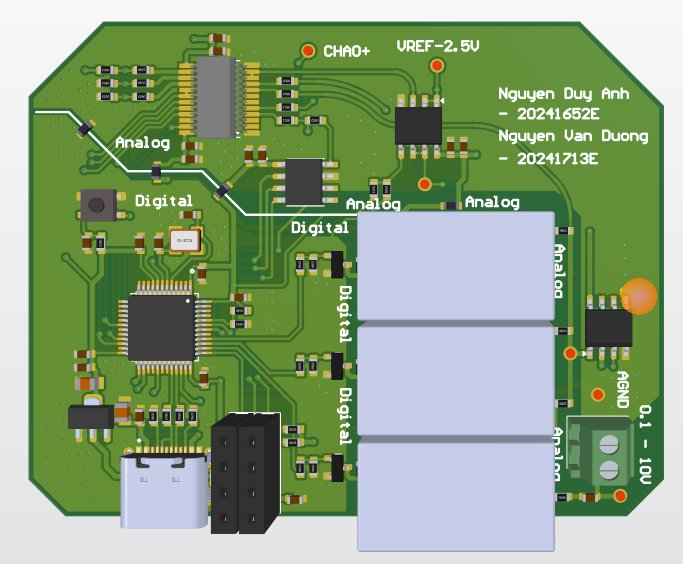
\includegraphics[width=\linewidth]{images/product/layout.png}
\\[-1mm]\small (a) Mô hình 3D có linh kiện
\end{minipage}\hfill
\begin{minipage}[t]{0.49\textwidth}
\centering
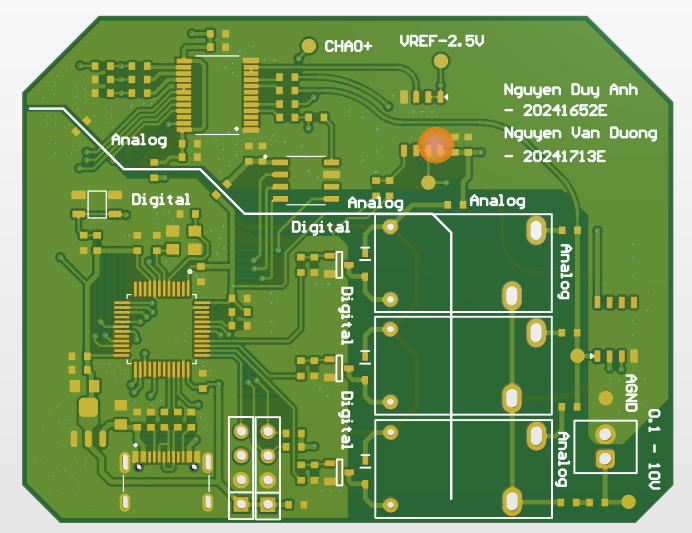
\includegraphics[width=\linewidth]{images/product/layout2.png}
\\[-1mm]\small (b) Bề mặt PCB và footprint
\end{minipage}
\caption{Mô hình bố trí PCB của thiết bị phân tích}
\label{fig:pcb_3d}
\end{figure}

\begin{figure}[H]
\centering
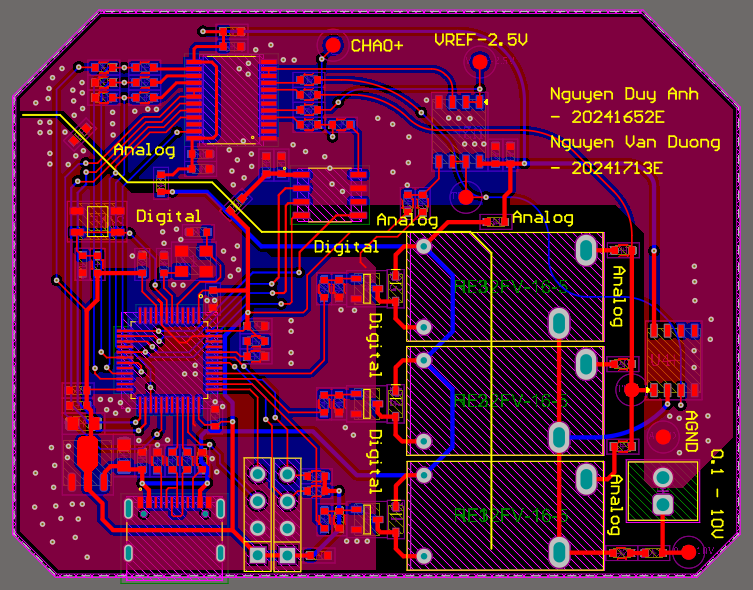
\includegraphics[width=0.88\textwidth]{images/product/layout3.png}
\caption{Layout các lớp đồng, via và vùng đổ đồng của PCB}
\label{fig:pcb_layout}
\end{figure}

Hình \ref{fig:pcb_product} là bo mạch đã lắp ráp dùng trong các thử nghiệm USB, DAC và ADC bring-up. Dây nối và phần gia cố quanh khu vực USB/MCU phản ánh trạng thái prototype đang debug, chưa phải hình thức cơ khí cuối cùng. Ảnh xác nhận bo đã được chế tạo, nhưng không thay thế phép đo continuity, nguồn, reference và timing cần thiết để xác nhận chuỗi analog.

\begin{figure}[H]
\centering

\includegraphics[width=0.72\textwidth]{images/product/product.png}
\caption{Bo mạch nguyên mẫu đã lắp ráp trong quá trình debug}
\label{fig:pcb_product}
\end{figure}

\chapter{THIẾT KẾ FIRMWARE VÀ GIAO THỨC TRUYỀN THÔNG}

\section{Kiến trúc firmware STM32F103}
Firmware được xây dựng bằng STM32Cube HAL và PlatformIO. Các thành phần chính gồm driver \code{mcp4822}, driver \code{ads7861}, \code{range\_control}, \code{calibration}, \code{measurement\_engine}, \code{test\_controller}, \code{command\_parser}, \code{protocol} và lớp USB Device CDC.

Sau khởi tạo clock và GPIO, firmware khởi tạo SPI1/SPI2 trong chế độ thường, ép USB re-enumeration, khởi động USB, nạp calibration và đưa hệ thống về IDLE. Callback nhận USB chỉ đưa từng byte vào parser; việc thực thi lệnh và tạo phản hồi diễn ra trong vòng lặp chính, tránh giữ ngắt USB quá lâu.

\section{Điều khiển MCP4822 và ADS7861}
Driver MCP4822 tạo frame 16-bit theo datasheet và truyền bằng SPI1--DMA. Bit kênh cho phép mở rộng sang hai đầu ra; bit gain điều khiển X1/X2. Driver ADS7861 tạo xung chuyển đổi theo timer và nhận hai word 16-bit bằng SPI2--DMA. Callback ngắt chủ yếu cập nhật cờ/trạng thái buffer; kết quả được chuẩn hóa về mã offset-binary 12-bit ở luồng xử lý trước khi truyền lên máy tính.

Trong chế độ NORMAL, lệnh \code{START} khởi tạo pipeline phát/thu liên tục. Buffer ADC được tổ chức theo khối để một khối có thể được xử lý và gửi USB trong khi DMA điền khối kế tiếp; độ trễ tăng theo kích thước buffer nhưng không làm thay đổi nhịp lấy mẫu. Trong chế độ USB SIM, phần cứng analog được bỏ qua; firmware tạo hai kênh sine có gain 0,8 và lệch pha $-25^\circ$. Các giá trị này chỉ dùng kiểm tra transport/DSP, không đại diện cho DUT thật.

\section{Thu thập, xử lý kết quả và calibration}
Measurement engine tính mean, Vpp, RMS AC, gain dB và phase. Trên desktop, các phép đo được thực hiện lại từ dữ liệu thô bằng sine fit để ổn định hơn khi số điểm trên chu kỳ thấp. Trục thời gian dùng tốc độ thực tế do firmware báo về thay vì chỉ dùng giá trị người dùng yêu cầu. Dù vậy, tại $20\unit{kHz}$ chỉ có khoảng 7 mẫu/chu kỳ nên các đại lượng phụ thuộc vị trí mẫu vẫn cần được đối chiếu với thiết bị chuẩn.

Calibration gồm hệ số DAC $(a,b)$ và các cặp $(m,c)$ cho từng kênh/từng range. Trên STM32F103, cấu trúc calibration được lưu tại trang Flash cuối, địa chỉ \code{0x0800FC00}. Các lệnh GET/SET/SAVE/RESET cho phép ứng dụng đọc, sửa và lưu hệ số mà không cần biên dịch lại firmware.

\section{USB CDC và giao thức lệnh}
Thiết bị sử dụng VID \code{0x0483}, PID \code{0x5740} và được Windows nhận bằng driver \code{usbser.sys}. USB chạy Full Speed; tốc độ baud $115200$ trong line coding chỉ là metadata của CDC, không giới hạn bus USB.

Trong quá trình phát triển, thiết bị từng xuất hiện COM nhưng báo Code 10. Nguyên nhân là vùng cấp phát tĩnh 512 byte nhỏ hơn cấu trúc \code{USBD\_CDC\_HandleTypeDef}. Sau khi vùng nhớ được xác định trực tiếp theo \code{sizeof}, class CDC khởi tạo thành công. Đồng thời, PMA được bố trí từ địa chỉ \code{0x40} trở lên để không chồng Buffer Descriptor Table, và ngắt \code{USB\_LP\_CAN1\_RX0} gọi đúng \code{HAL\_PCD\_IRQHandler}.

\begin{table}[H]
\centering
\caption{Các lệnh chính của giao thức ASCII}
\label{tab:commands}
\begin{tabularx}{\textwidth}{|p{3.5cm}|p{3.2cm}|X|}
\hline
\tableheadcolor\textbf{Lệnh} & \textbf{Phản hồi} & \textbf{Chức năng} \\ \hline
PING & OK & Kiểm tra kết nối hai chiều \\ \hline
INFO & DATA:... & Đọc tên thiết bị và phiên bản firmware \\ \hline
CONFIG:... & OK/ERR & Cấu hình dạng sóng, $f$, biên độ, offset, gain, $F_s$, số mẫu \\ \hline
START / STOP & OK & Bắt đầu hoặc dừng phép đo \\ \hline
GET\_STATUS & DATA:IDLE/\newline RUNNING & Đọc trạng thái bộ điều khiển \\ \hline
GET\_RESULT & RESULT:\{...\} & Nhận kết quả dạng JSON một dòng \\ \hline
GET\_SAMPLES & Binary frame & Nhận mẫu CH1/CH2 \\ \hline
SET\_RANGE /\newline GET\_RANGE & OK/DATA & Điều khiển và đọc range \\ \hline
GET/SET/\newline SAVE\_CALIB & DATA/OK & Quản lý hệ số hiệu chuẩn \\ \hline
\end{tabularx}
\end{table}

\section{Giao thức truyền dữ liệu nhị phân}
Khung dữ liệu mẫu được mô tả trong Bảng \ref{tab:binaryframe}. Payload chứa các cặp CH1/CH2, mỗi mẫu 16-bit big-endian nhưng chỉ sử dụng 12 bit thấp. Với 512 cặp mẫu, payload dài 2048 byte.

\begin{table}[H]
\centering
\caption{Cấu trúc frame dữ liệu mẫu}
\label{tab:binaryframe}
\begin{tabularx}{\textwidth}{|p{3.5cm}|p{3cm}|X|}
\hline
\tableheadcolor\textbf{Trường} & \textbf{Kích thước} & \textbf{Giá trị/ý nghĩa} \\ \hline
Header & 2 byte & \code{0xAA 0xBB} \\ \hline
Frame type & 1 byte & \code{0x03} cho OSC capture \\ \hline
Payload length & 2 byte & Big-endian \\ \hline
Payload & $4M$ byte & $M$ cặp CH1/CH2 \\ \hline
Checksum & 1 byte & XOR toàn payload \\ \hline
\end{tabularx}
\end{table}

Firmware gửi payload theo chunk 64 byte để phù hợp packet USB FS và chờ \code{TxState} hoàn tất trước khi tái sử dụng buffer. Desktop đọc đủ đúng số byte, kiểm header, type, length và checksum. Frame thiếu hoặc sai checksum được chuyển thành lỗi truyền thông thay vì đưa vào DSP.

\section{Tài nguyên và các chế độ kiểm thử}
PlatformIO định nghĩa các environment \code{production}, \code{usb\_cdc\_test} và \code{mcp4822\_test}. Source còn khai báo các mode kiểm tra ADC, SPI loopback và Flash calibration, nhưng không phải tất cả đều có environment PlatformIO độc lập hoặc đã được xác nhận build. Kết quả build production được xác nhận gần nhất trước các chỉnh sửa chẩn đoán ADC ngày 17/07/2026 được trình bày trong Bảng \ref{tab:resource}; cần build lại để chốt số liệu của source mới hơn.

\begin{table}[H]
\centering
\caption{Tài nguyên firmware production được xác nhận gần nhất}
\label{tab:resource}
\begin{tabularx}{\textwidth}{|p{3.1cm}|Y|Y|Y|Y|}
\hline
\tableheadcolor\textbf{Environment} & \textbf{RAM (byte)} & \textbf{RAM} & \textbf{Flash (byte)} & \textbf{Flash} \\ \hline
Production (16/07/2026) & 8.968/20.480 & 43,8\% & 49.932/65.536 & 76,2\% \\ \hline
\end{tabularx}
\end{table}
Dung lượng nằm trong giới hạn của STM32F103C8T6 và còn khoảng 56,2\% SRAM tại lần build đã xác nhận. Firmware vẫn tránh mảng float lớn và dùng buffer tĩnh có kích thước xác định. Các artifact build được lưu trong repository không được dùng thay cho kết quả build lại từ source hiện hành.

\chapter{THIẾT KẾ ỨNG DỤNG DESKTOP VÀ XỬ LÝ TÍN HIỆU}

\section{Kiến trúc ứng dụng Signal Analyzer Pro}
Ứng dụng được phát triển bằng Python 3, PyQt6 và PyQtGraph \cite{pyqt,pyqtgraph}. NumPy/SciPy thực hiện xử lý số; PySerial cung cấp giao tiếp COM \cite{numpy,scipy,pyserial}. Kiến trúc gồm ba phần: lớp UI/controller trong \code{signal\_analyzer.py}, worker đọc USB và module \code{signal\_analysis.py} chứa các công thức có thể kiểm thử độc lập.

Các tab điều khiển gồm Network Analyzer, Bode Sweep, Calibration và Passive Oscilloscope. Các tab hiển thị gồm Oscilloscope Monitor, Frequency Sweep và Measurements. Thiết kế giữ giao diện thao tác tập trung nhưng tách DSP ra khỏi code widget nhằm tránh lặp công thức.

Hình \ref{fig:appwave} là ảnh chụp ứng dụng khi đo phần cứng thật tại $100\unit{Hz}$, với tốc độ lấy mẫu thực tế $140{,}077\unit{SPS}$. Hai kênh Vin/Vout có dạng sine rõ ràng, cho phép quan sát trực tiếp mức điện áp, độ khuếch đại và trạng thái kết nối COM4.

\begin{figure}[H]
\centering
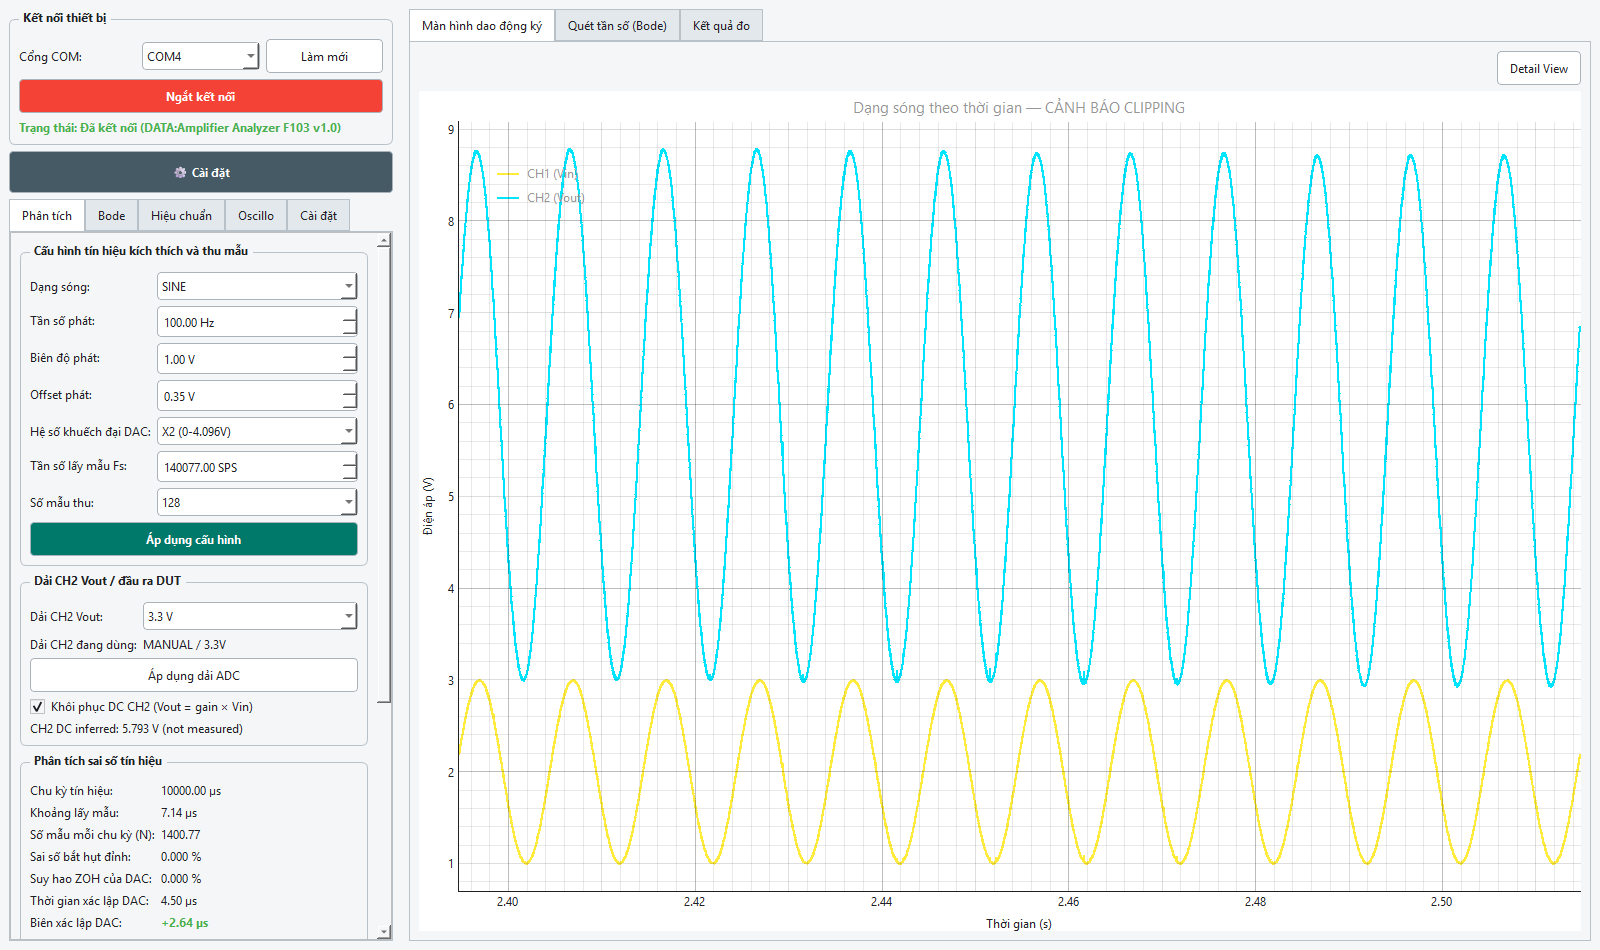
\includegraphics[width=0.95\textwidth]{images/result_app/01_freq_100hz_waveform.png}
\caption{Giao diện waveform khi đo phần cứng thật tại $100\unit{Hz}$}
\label{fig:appwave}
\end{figure}

\section{Giao diện và luồng giao tiếp USB}
Khi kết nối, ứng dụng quét danh sách COM, mở cổng, xóa buffer, gửi PING tối đa ba lần, sau đó đọc INFO và range. Khi đo live, QTimer chỉ khởi tạo worker nếu worker trước đã hoàn tất. Worker gửi GET\_RESULT và GET\_SAMPLES, đọc frame với timeout rồi phát signal về main thread. Vì vậy mất cổng hoặc thiếu byte không khóa cửa sổ.

\section{Phân tích điều kiện lấy mẫu và sai số DAC}
Hàm \code{calculate\_sampling\_quality} là nguồn duy nhất cho Period, Sample Interval, $N$, peak error, ZOH droop và settling margin. Ngưỡng đánh giá gồm:
\begin{itemize}
    \item $N<10$: WARNING\_SAMPLE\_TOO\_LOW;
    \item $10\leq N<25$: WARNING\_POC\_ONLY;
    \item $E_{peak}>1\%$: cảnh báo sai số peak;
    \item $T_{margin}<0$: DAC chưa xác lập;
    \item $0\leq T_{margin}<1\unit{\mu s}$: borderline.
\end{itemize}
Các giá trị cấu hình được cập nhật ngay khi người dùng thay đổi $f$ hoặc $F_s$, không cần chờ chạy phép đo.

\section{Phân tích tín hiệu CH1 và CH2}
Mỗi kênh được tính Vmax, Vmin, Vpp, Vpeak, RMS toàn phần, RMS AC, mean, tần số, chu kỳ và noise residual. Tần số ban đầu được ước lượng bằng positive zero crossing có nội suy phân đoạn. Sine fit tại tần số mục tiêu giải hệ tuyến tính gồm sin, cos và hằng số, từ đó suy ra amplitude, offset, phase và RMS phần dư.

Clipping được phát hiện khi có plateau ít nhất ba mẫu liên tiếp gần cực trị; saturation được phát hiện trực tiếp từ raw code gần 0 hoặc 4095. Quy tắc ba mẫu tránh nhận nhầm hai điểm đỉnh bằng nhau trong trường hợp lấy 10 mẫu/chu kỳ.

\section{Phân tích DUT và PASS/FAIL/WARNING}
Ứng dụng ưu tiên $V_{RMS,AC}$ để tính gain và dùng phase sine-fit của CH2 trừ CH1. Gain error được so sánh với target/tolerance. Tần số và biên độ vào cũng có tolerance riêng. Communication error, data loss, clipping và saturation là điều kiện FAIL. Nếu các spec đạt nhưng sampling quality có cảnh báo, kết quả cuối là WARNING.

Hình \ref{fig:appmeasure} trình bày bảng Channel Measurement và DUT Analysis của cùng phép đo phần cứng. Ứng dụng xác định tần số hai kênh xấp xỉ $99{,}984\unit{Hz}$, gain đo được 2,889 lần, tương đương $9{,}214\unit{dB}$. Các cờ clipping và gain ngoài dung sai vẫn được giữ nguyên trong ảnh để phản ánh trung thực cấu hình đánh giá tại thời điểm chụp.

\begin{figure}[H]
\centering
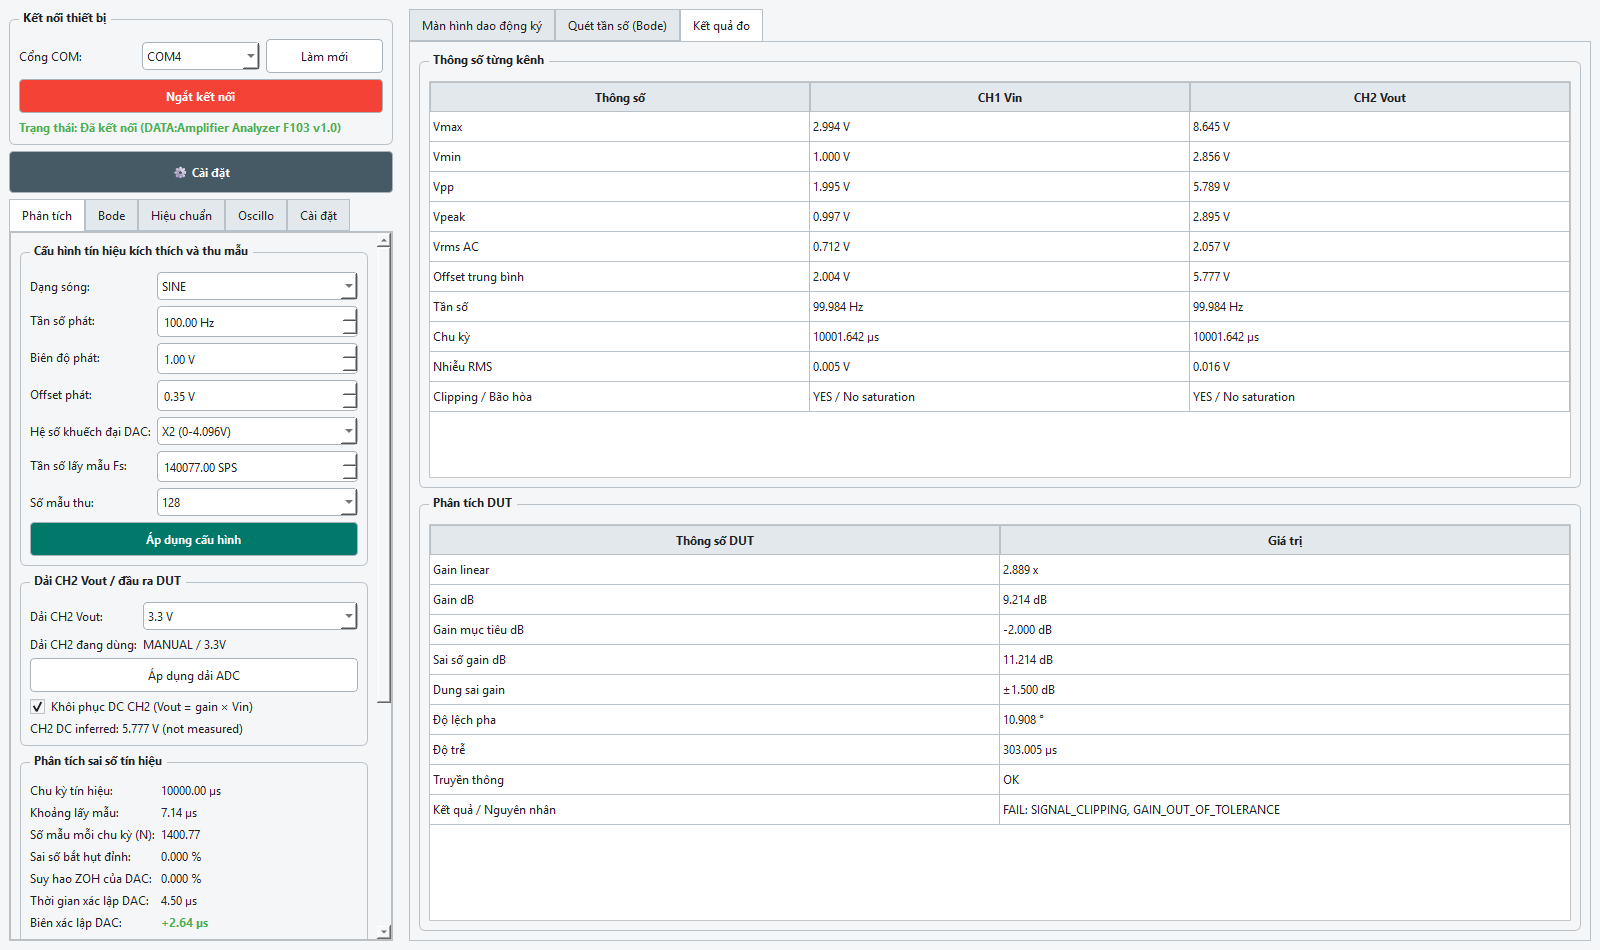
\includegraphics[width=0.95\textwidth]{images/result_app/01_freq_100hz_results.png}
\caption{Bảng thông số từng kênh và phân tích DUT từ phép đo phần cứng thật}
\label{fig:appmeasure}
\end{figure}

\section{Calibration, simulation và xuất dữ liệu}
Tab Calibration hiển thị trạng thái default, loaded from device, loaded from JSON, modified but not saved hoặc saved to device. Người dùng có thể đọc/ghi hệ số qua USB và import/export JSON. Việc chuyển raw ADC sang volt trên desktop sử dụng cùng mô hình scale/offset theo range như firmware.

Khi không có thiết bị, mục SIMULATE tạo cặp sine Vin/Vout theo đúng $F_s$, số mẫu, gain và phase. Chế độ này cho phép kiểm tra UI, DSP và export độc lập với phần cứng. Báo cáo JSON chứa timestamp, device info, cấu hình waveform, sampling quality, channel metrics, DUT metrics, calibration, trạng thái truyền thông và kết quả. Nếu người dùng chọn, raw samples được lưu đồng thời trong CSV và JSON.

\chapter{KIỂM NGHIỆM, KẾT QUẢ VÀ THẢO LUẬN}

\section{Cấu hình và phương pháp kiểm nghiệm}
Kiểm nghiệm được chia thành bốn lớp: unit test cho công thức, kiểm tra giao tiếp USB trên bo STM32F103, kiểm tra tích hợp desktop với firmware USB SIM và kiểm tra chuỗi analog thật. Thiết bị được nạp bằng J-Link; bộ kết quả mới nhất được thu trực tiếp trên \textit{USB Serial Device (COM4)} bằng ứng dụng Signal Analyzer Pro. Firmware được đặt $F_s=140\unit{kSPS}$ và ứng dụng ghi nhận tốc độ thực tế $140{,}077\unit{SPS}$. Ma trận thử gồm quét tần số từ $100\unit{Hz}$ đến $20\unit{kHz}$ với tín hiệu $2\pm1\unit{V}$, sau đó thay đổi biên độ và dải đo. Tất cả hình trong các Mục \ref{sec:real_frequency} và \ref{sec:real_range} là ảnh chụp màn hình ứng dụng khi chạy phần cứng thật, không phải dữ liệu mô phỏng.

\subsection{Module DUT thử nghiệm}
Hình \ref{fig:dut_module} trình bày schematic và module DUT rời được chuẩn bị để thử chuỗi phát/thu. Mạch sử dụng NE5532AP, có đầu nối nguồn $12\unit{V}$, mass analog, ngõ vào và ngõ ra. Hai điện trở dùng để đặt gain có giá trị $R_f=R4=20\,\mathrm{k}\Omega$ và $R_g=R34=10\,\mathrm{k}\Omega$.

Với topology khuếch đại không đảo dự kiến, tín hiệu phải được đưa vào đầu $(+)$; $R_f$ nối từ OUT về đầu $(-)$ và $R_g$ nối từ đầu $(-)$ xuống mass. Khi op-amp làm việc trong vùng tuyến tính và có hồi tiếp âm, gain điện áp vòng kín là:
\begin{equation}
A_v=\frac{V_{out}}{V_{in}}=1+\frac{R_f}{R_g}
   =1+\frac{20\,\mathrm{k}\Omega}{10\,\mathrm{k}\Omega}=3.
\label{eq:dut_gain_linear}
\end{equation}
Gain theo decibel tương ứng:
\begin{equation}
G_{dB}=20\log_{10}|A_v|=20\log_{10}(3)\approx 9{,}54\unit{dB}.
\label{eq:dut_gain_db}
\end{equation}
Do đó, khi kiểm thử đúng topology này, giá trị mục tiêu trên ứng dụng nên đặt $A_v=3$ hoặc $G_{target}=9{,}54\unit{dB}$. Ví dụ, với sine đầu vào có biên độ đỉnh $0{,}3\unit{V}$, đầu ra lý tưởng có biên độ đỉnh $0{,}9\unit{V}$, miễn là nguồn cấp và output swing của NE5532 không gây clipping.

Sơ đồ mô phỏng trong Hình \ref{fig:dut_module}(a) từng gây nhầm lẫn về cực tính hồi tiếp, do đó kết nối thực tế đã được kiểm tra lại bằng oscilloscope. Kết quả ở Hình \ref{fig:oscillo_dut_200hz} cho thấy đầu ra DUT vẫn là sine, cùng tần số với đầu ra DAC và có biên độ lớn hơn. Bằng chứng thực nghiệm này xác nhận module đang làm việc trong vùng khuếch đại đối với cấu hình dây đo hiện tại. Giá trị gain định lượng vẫn phải lấy từ dữ liệu đã hiệu chuẩn thay vì chỉ suy ra từ số ô chia trên màn hình oscilloscope.

\begin{figure}[H]
\centering
\begin{minipage}[t]{0.49\textwidth}
\centering
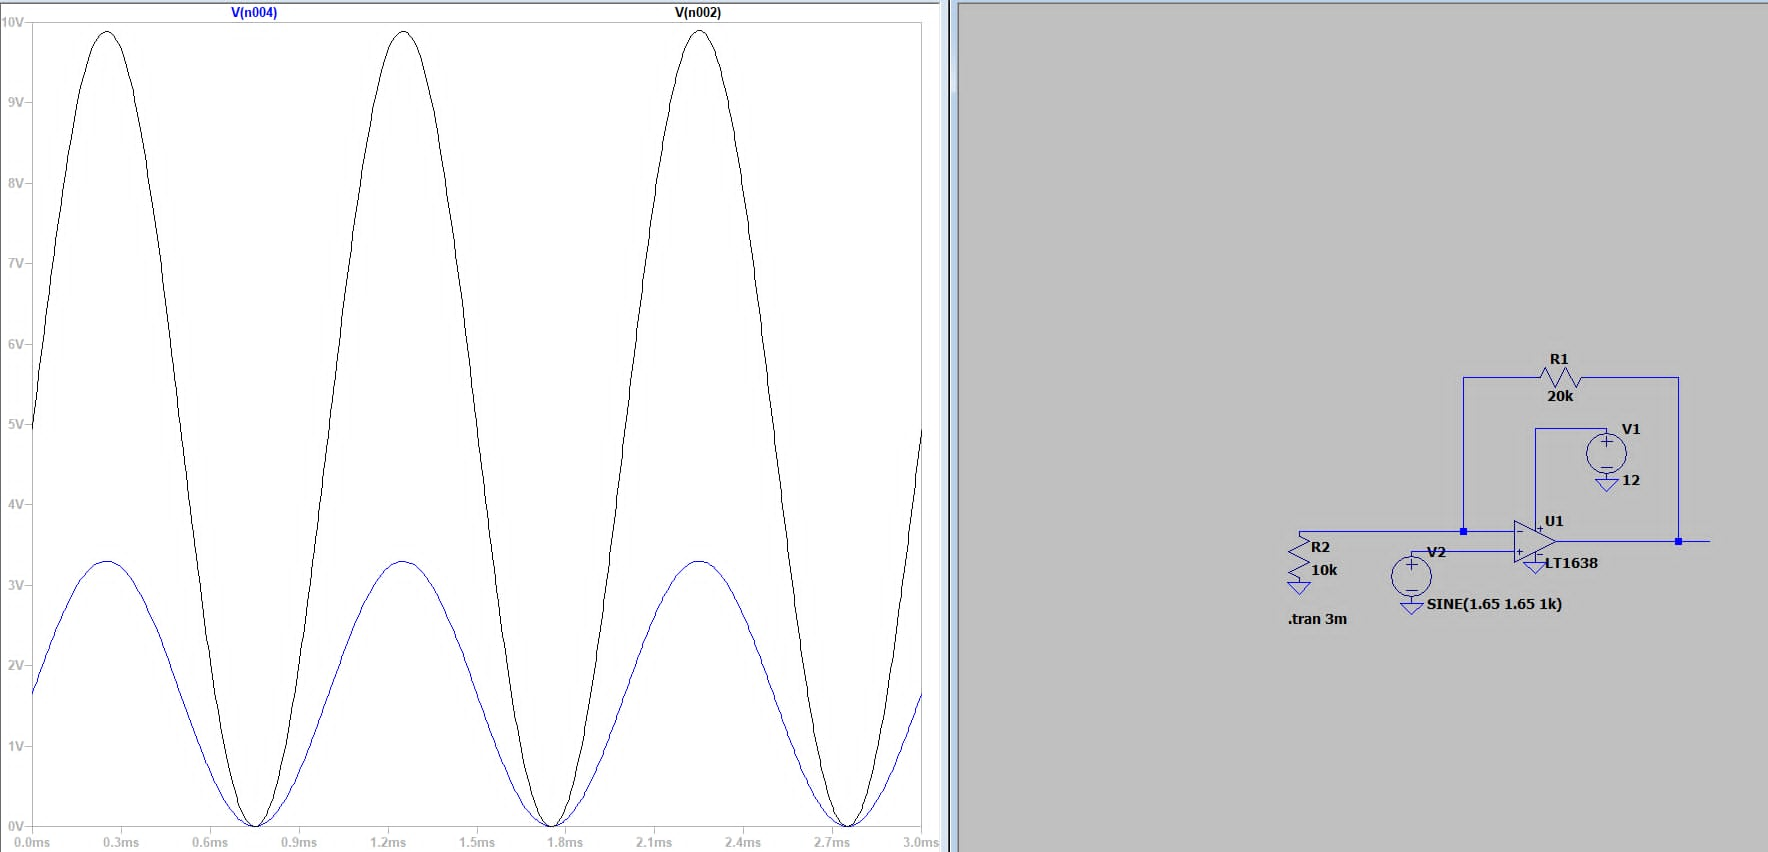
\includegraphics[width=\linewidth]{images/DUT/simulate.png}
\\[-1mm]\small (a) Sơ đồ và kết quả mô phỏng DUT
\end{minipage}\hfill
\begin{minipage}[t]{0.49\textwidth}
\centering
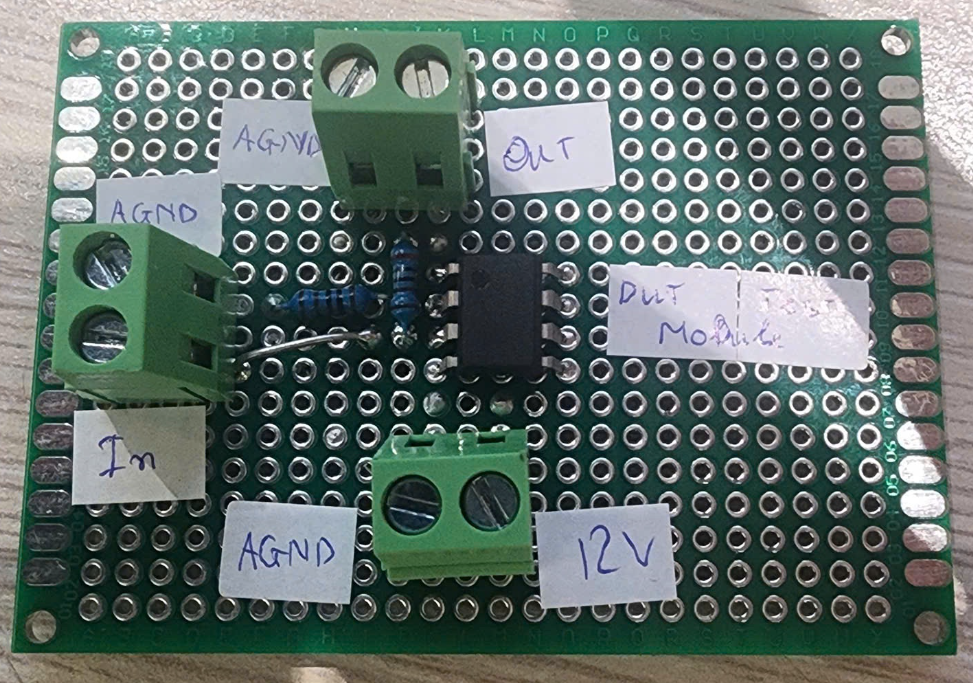
\includegraphics[width=\linewidth]{images/DUT/product.png}
\\[-1mm]\small (b) Module DUT lắp trên board thử
\end{minipage}
\caption{Module DUT sử dụng trong quá trình thử nghiệm phần cứng}
\label{fig:dut_module}
\end{figure}

\subsection{Xác nhận chuỗi DAC--DUT bằng oscilloscope}
Để kiểm tra độc lập với ADC và phần mềm desktop, hai đầu dò oscilloscope được nối đồng thời vào đầu ra DAC và đầu ra DUT. Ứng dụng được cấu hình phát sine $200\unit{Hz}$, biên độ đặt $1{,}00\unit{V}$, offset $0{,}50\unit{V}$, DAC ở chế độ X2, $F_s=140{,}077\unit{SPS}$ và khối thu 128 mẫu. Trên Hình \ref{fig:oscillo_dut_200hz}, đường màu vàng là đầu ra DAC và đường màu tím là đầu ra DUT.

\begin{figure}[H]
\centering

\includegraphics[width=0.92\textwidth]{images/oscillo/image.png}
\caption{Đo đồng thời đầu ra DAC (màu vàng) và đầu ra DUT (màu tím) tại $200\unit{Hz}$}
\label{fig:oscillo_dut_200hz}
\end{figure}

Thang thời gian hiển thị là $2{,}5\unit{ms/div}$, nên một chu kỳ chiếm xấp xỉ hai ô, phù hợp với chu kỳ lý thuyết $T=1/200=5\unit{ms}$. Hai tín hiệu giữ cùng tần số và gần như cùng pha; biên độ đầu ra DUT lớn hơn rõ rệt so với đầu ra DAC. Quan sát này là bằng chứng độc lập rằng khối phát DAC và module DUT hoạt động end-to-end trước khi tín hiệu được đưa vào AFE/ADC. Do ảnh chụp dùng để xác nhận chức năng và vị trí zero của hai kênh khác nhau, không dùng trực tiếp ảnh này để công bố gain chính xác.

\section{Kiểm nghiệm USB CDC}
Kết quả kiểm nghiệm USB được tóm tắt trong Bảng \ref{tab:usbtest}. Thiết bị có trạng thái \code{CM\_PROB\_NONE}; request/response ASCII và binary đều hoạt động.

\begin{table}[H]
\centering
\caption{Kết quả kiểm nghiệm USB CDC}
\label{tab:usbtest}
\begin{tabularx}{\textwidth}{|p{4.5cm}|X|p{1.9cm}|}
\hline
\tableheadcolor\textbf{Phép thử} & \textbf{Kết quả quan sát} & \textbf{Đánh giá} \\ \hline
Enumeration & COM4, VID:PID=0483:5740, thiết bị hoạt động & PASS \\ \hline
PING/INFO & PING$\rightarrow$OK; INFO trả đúng tên firmware & PASS \\ \hline
Chu kỳ protocol đầy đủ & 20/20 chu kỳ STOP--RANGE--CONFIG--START--RESULT--SAMPLES--PING & PASS \\ \hline
Chu kỳ kiểu live & 30/30 JSON hợp lệ, frame đủ và checksum đúng & PASS \\ \hline
Frame 128 mẫu/kênh & 512 byte payload, header/type đúng, checksum đúng & PASS \\ \hline
STOP/GET\_STATUS & Trạng thái cuối DATA:IDLE & PASS \\ \hline
\end{tabularx}
\end{table}

\section{Kiểm nghiệm điều kiện lấy mẫu}
Bốn test case bắt buộc được chạy bằng unit test và kiểm tra lại trên UI. Kết quả ở Bảng \ref{tab:samplingcases} khớp công thức lý thuyết.

\begin{table}[H]
\centering
\caption{Kết quả đánh giá các cấu hình lấy mẫu}
\label{tab:samplingcases}
\begin{tabularx}{\textwidth}{|p{1.8cm}|p{2cm}|p{0.8cm}|p{1.7cm}|p{1.7cm}|X|}
\hline
\tableheadcolor$f$ & $F_s$ & $N$ & $E_{peak}$ & $E_{ZOH}$ & $T_{margin}$ / Kết luận \\ \hline
$20\unit{kHz}$ & $200\unit{kSPS}$ & 10 & 4,894\% & 1,637\% & $+0,50\unit{\mu s}$; POC \\ \hline
$20\unit{kHz}$ & $500\unit{kSPS}$ & 25 & 0,789\% & 0,263\% & $-2,50\unit{\mu s}$; DAC chưa ổn định \\ \hline
$20\unit{kHz}$ & $1\unit{MSPS}$ & 50 & 0,197\% & 0,066\% & $-3,50\unit{\mu s}$; DAC chưa ổn định \\ \hline
$2\unit{kHz}$ & $200\unit{kSPS}$ & 100 & 0,049\% & 0,016\% & $+0,50\unit{\mu s}$; borderline \\ \hline
\end{tabularx}
\end{table}

Kết quả cho thấy tăng $F_s$ làm giảm sai số lấy mẫu nhưng không tự động cải thiện toàn hệ thống. Khi DAC cũng được cập nhật ở cùng tốc độ, khoảng thời gian mỗi mẫu có thể nhỏ hơn settling time. Vì vậy $500\unit{kSPS}$ và $1\unit{MSPS}$ có nhiều điểm/chu kỳ nhưng vẫn bị cảnh báo DAC not settled. Cách khắc phục là giảm tốc độ cập nhật DAC, dùng timer riêng, tạo LUT theo chu kỳ hoặc chọn DAC nhanh hơn.

Sau khi chuyển chuỗi thu sang kiến trúc timer--SPI--DMA và dùng buffer liên tục, tốc độ ADC không còn bị giới hạn bởi vòng đọc GPIO blocking trước đây. Trong đợt đo phần cứng trình bày dưới đây, tốc độ yêu cầu là $140\unit{kSPS}$ và tốc độ được firmware/ứng dụng báo lại là $140{,}077\unit{SPS}$. Như vậy số mẫu trên một chu kỳ giảm từ khoảng 1401 điểm ở $100\unit{Hz}$ xuống còn 7 điểm ở $20\unit{kHz}$. Tốc độ này đủ để nhận diện tín hiệu $20\unit{kHz}$ theo Nyquist, nhưng chưa đủ dư địa để tái tạo hình dạng, đỉnh và pha với độ tin cậy như ở vùng tần số thấp.

\section{Kết quả quét tần số trên phần cứng thật}
\label{sec:real_frequency}
Năm mức tần số đã được chạy tự động; báo cáo chọn ba mức đặc trưng thay vì đưa toàn bộ ảnh. Bảng \ref{tab:real_frequency_cases} thể hiện tiêu chí lựa chọn, bao gồm một trường hợp tốt, một trường hợp trung gian và một trường hợp bộc lộ giới hạn lấy mẫu.

\begin{table}[H]
\centering
\caption{Ba trường hợp đại diện của phép quét tần số thực tế}
\label{tab:real_frequency_cases}
\begin{tabularx}{\textwidth}{|p{2.3cm}|p{2.6cm}|p{2.4cm}|X|}
\hline
\tableheadcolor\textbf{Tần số} & \textbf{$F_s$ thực tế} & \textbf{Mẫu/chu kỳ} & \textbf{Vai trò trong đánh giá} \\ \hline
$100\unit{Hz}$ & $140{,}077\unit{SPS}$ & 1400,77 & Trường hợp tốt: dạng sóng trơn, mật độ mẫu lớn. \\ \hline
$5\unit{kHz}$ & $140{,}077\unit{SPS}$ & 28,02 & Trường hợp trung gian: vẫn nhận diện tốt chu kỳ nhưng ít điểm hơn rõ rệt. \\ \hline
$20\unit{kHz}$ & $140{,}077\unit{SPS}$ & 7,00 & Trường hợp giới hạn: waveform đa giác và các đại lượng đỉnh/pha nhạy với vị trí mẫu. \\ \hline
\end{tabularx}
\end{table}

\begin{figure}[H]
\centering
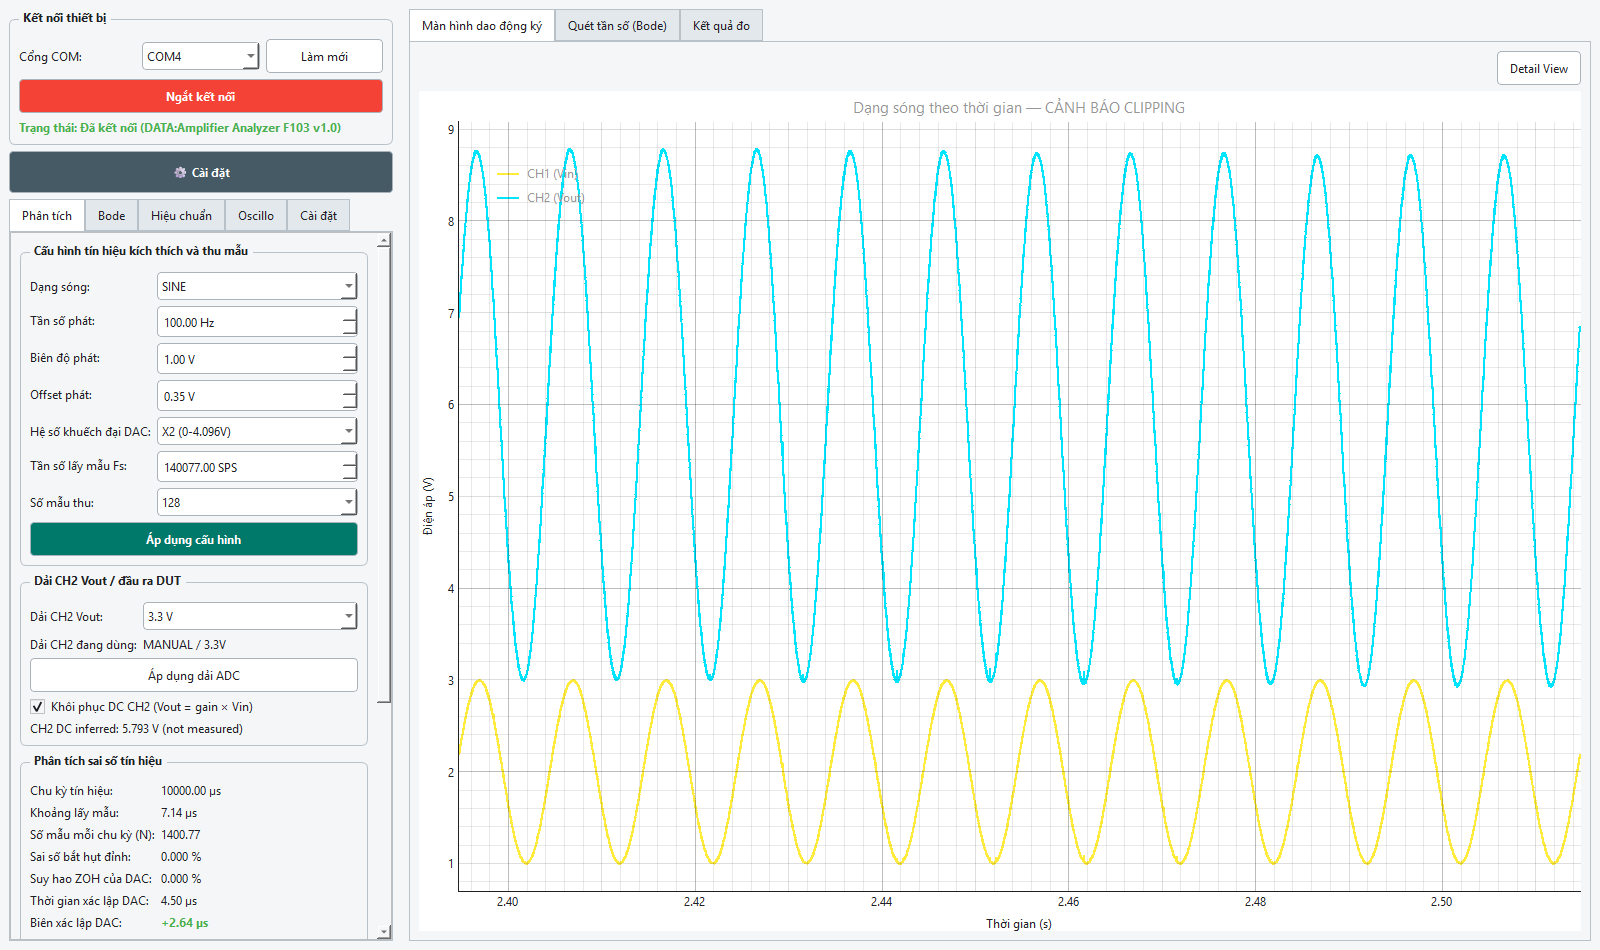
\includegraphics[width=0.82\textwidth]{images/result_app/01_freq_100hz_waveform.png}\\[2mm]
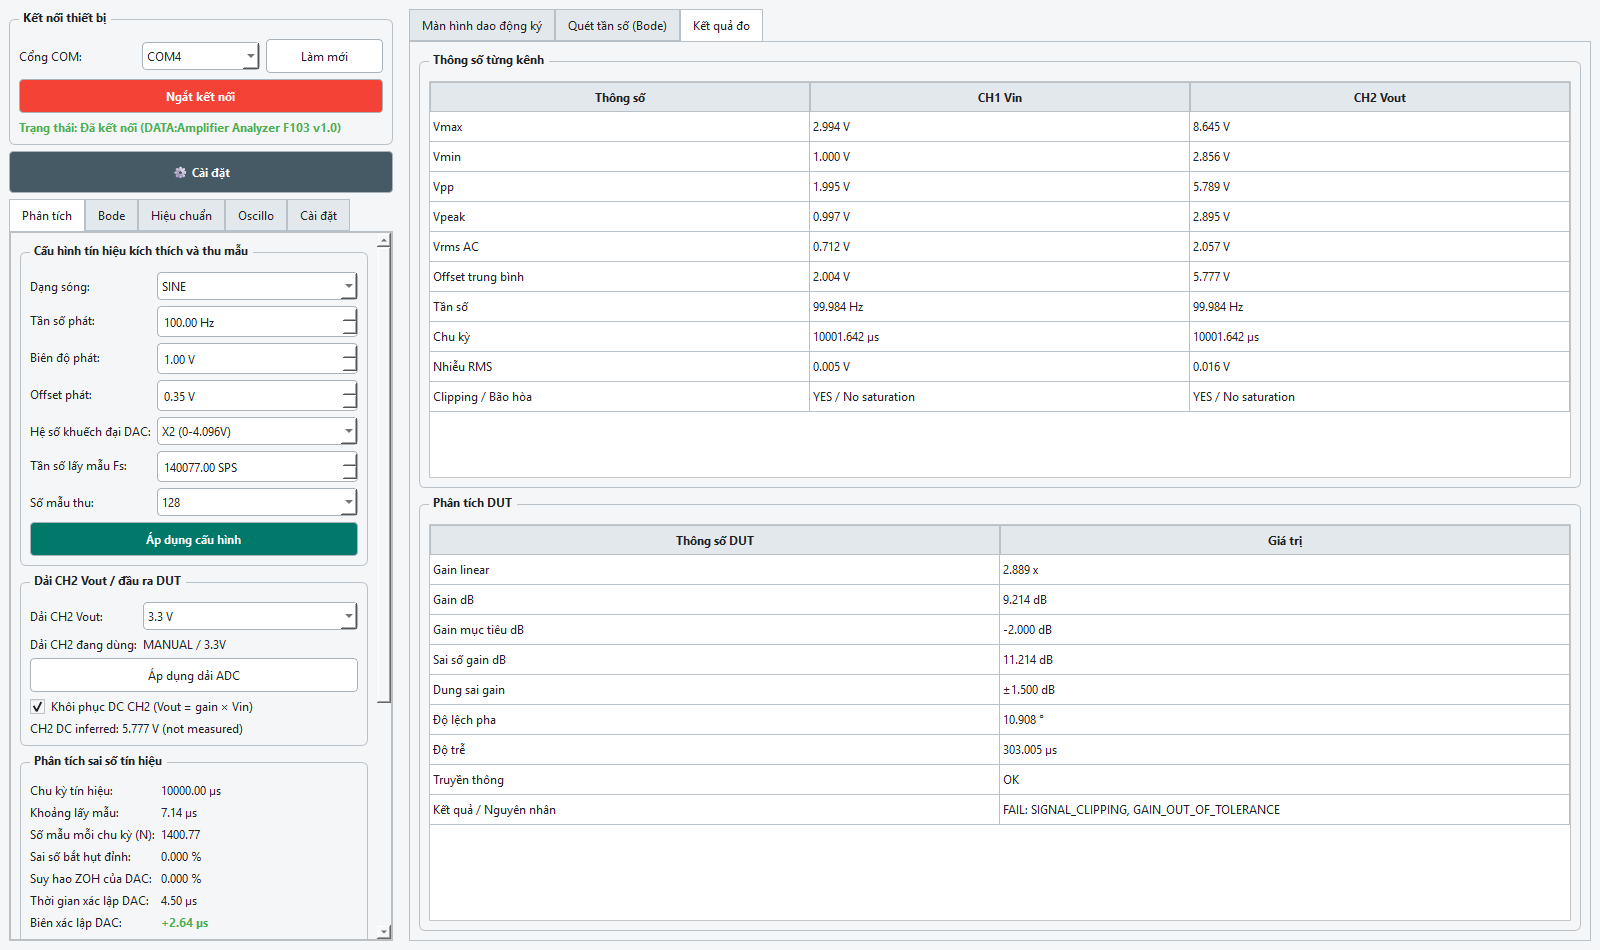
\includegraphics[width=0.82\textwidth]{images/result_app/01_freq_100hz_results.png}
\caption{Kết quả thực tế tại $100\unit{Hz}$: waveform (trên) và bảng thông số do ứng dụng tính toán (dưới)}
\label{fig:real_freq_100}
\end{figure}

Ở $100\unit{Hz}$, khoảng 1401 mẫu trên mỗi chu kỳ giúp đường nối mẫu gần với đường cong liên tục. Đây là trường hợp thuận lợi để quan sát biên độ, offset và kiểm tra kết nối toàn chuỗi DAC--DUT--ADC. Bảng kết quả được giữ nguyên để thể hiện cả các cảnh báo do ứng dụng phát hiện, thay vì chỉ lựa chọn phần dữ liệu đẹp.

\begin{figure}[H]
\centering
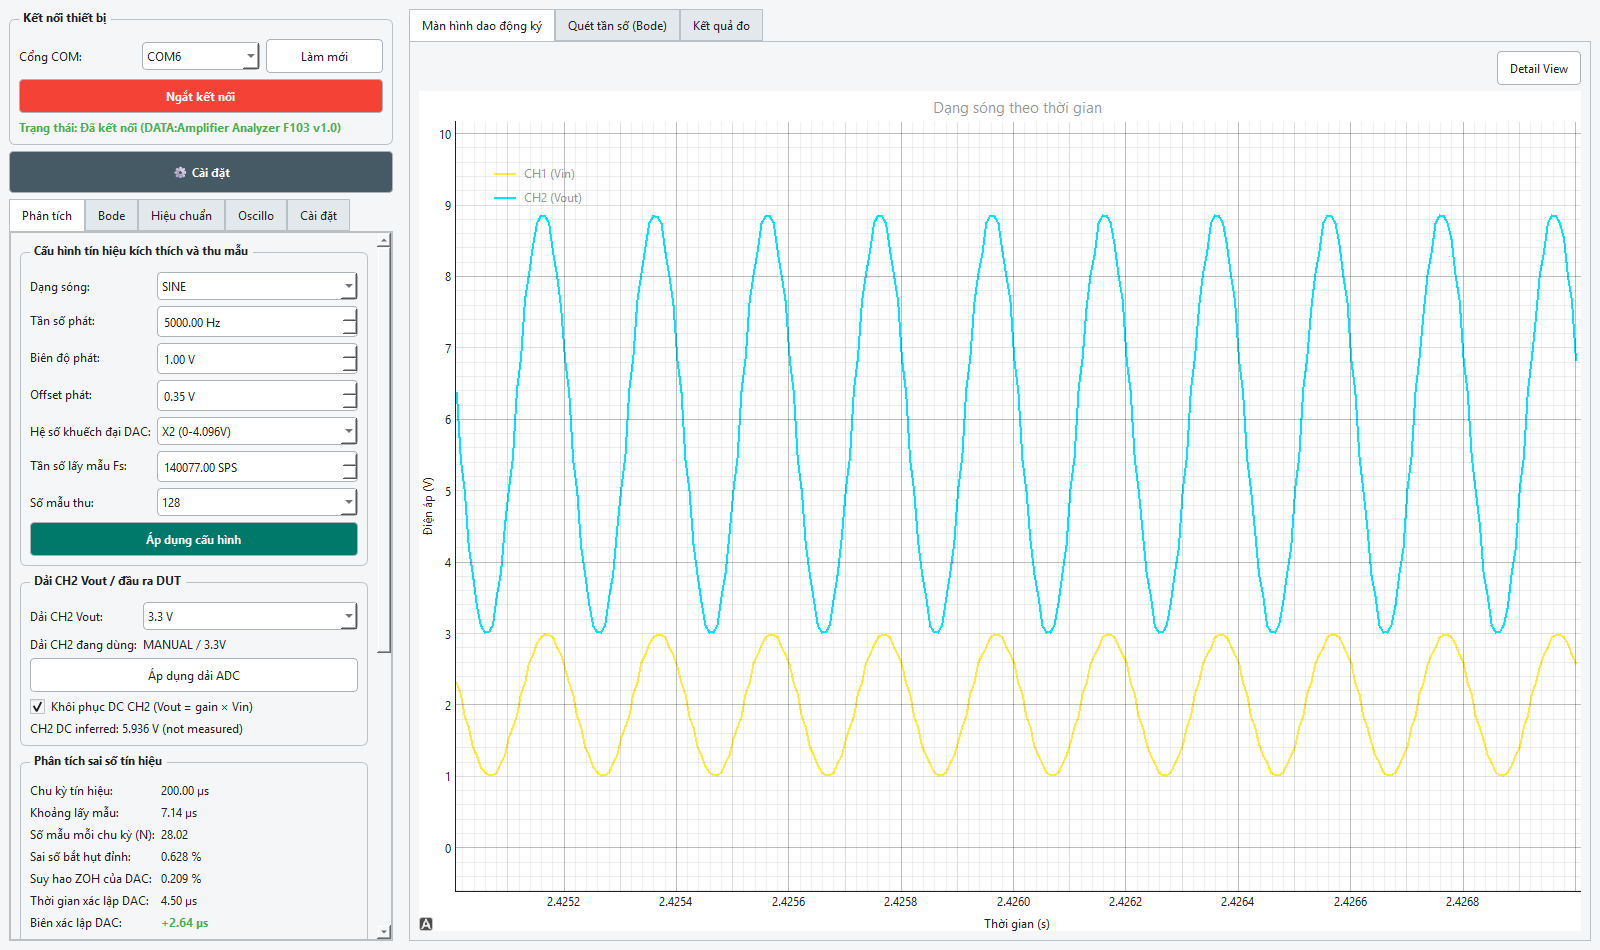
\includegraphics[width=0.82\textwidth]{images/result_app/03_freq_5000hz_waveform.png}\\[2mm]
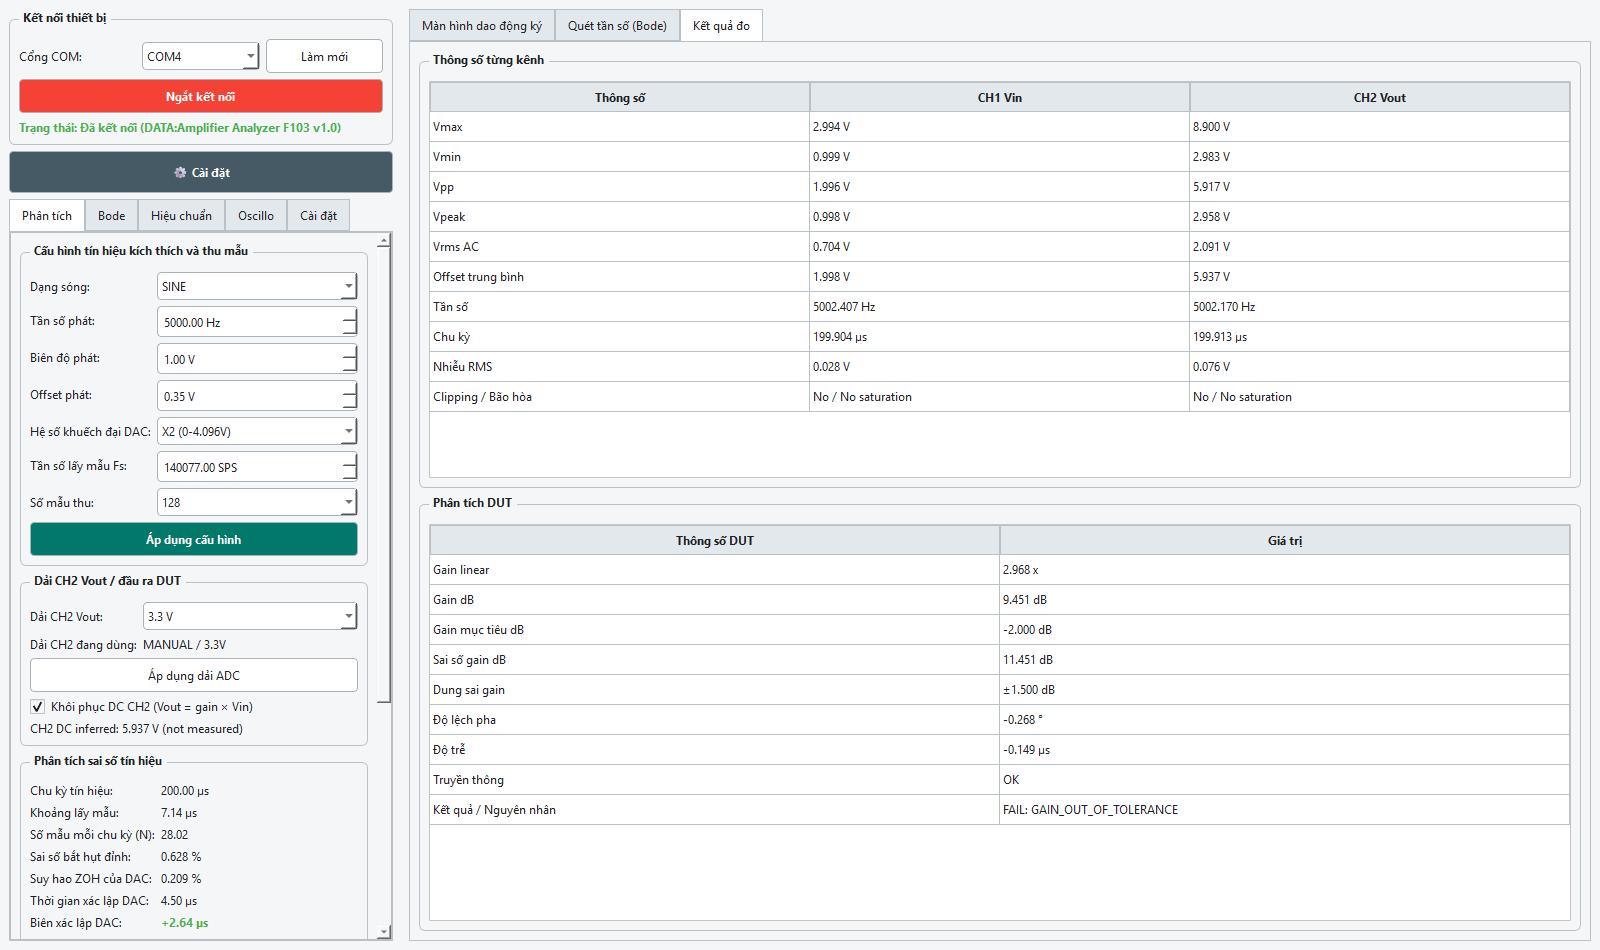
\includegraphics[width=0.82\textwidth]{images/result_app/03_freq_5000hz_results.png}
\caption{Kết quả thực tế tại $5\unit{kHz}$: waveform (trên) và bảng thông số (dưới)}
\label{fig:real_freq_5k}
\end{figure}

Tại $5\unit{kHz}$, số mẫu giảm còn khoảng 28 điểm mỗi chu kỳ. Dạng sóng vẫn thể hiện được tính tuần hoàn và quan hệ giữa hai kênh, nhưng độ mịn thấp hơn trường hợp $100\unit{Hz}$. Đây là vùng hoạt động trung gian hợp lý giữa tốc độ đo và chất lượng hiển thị.

\begin{figure}[H]
\centering
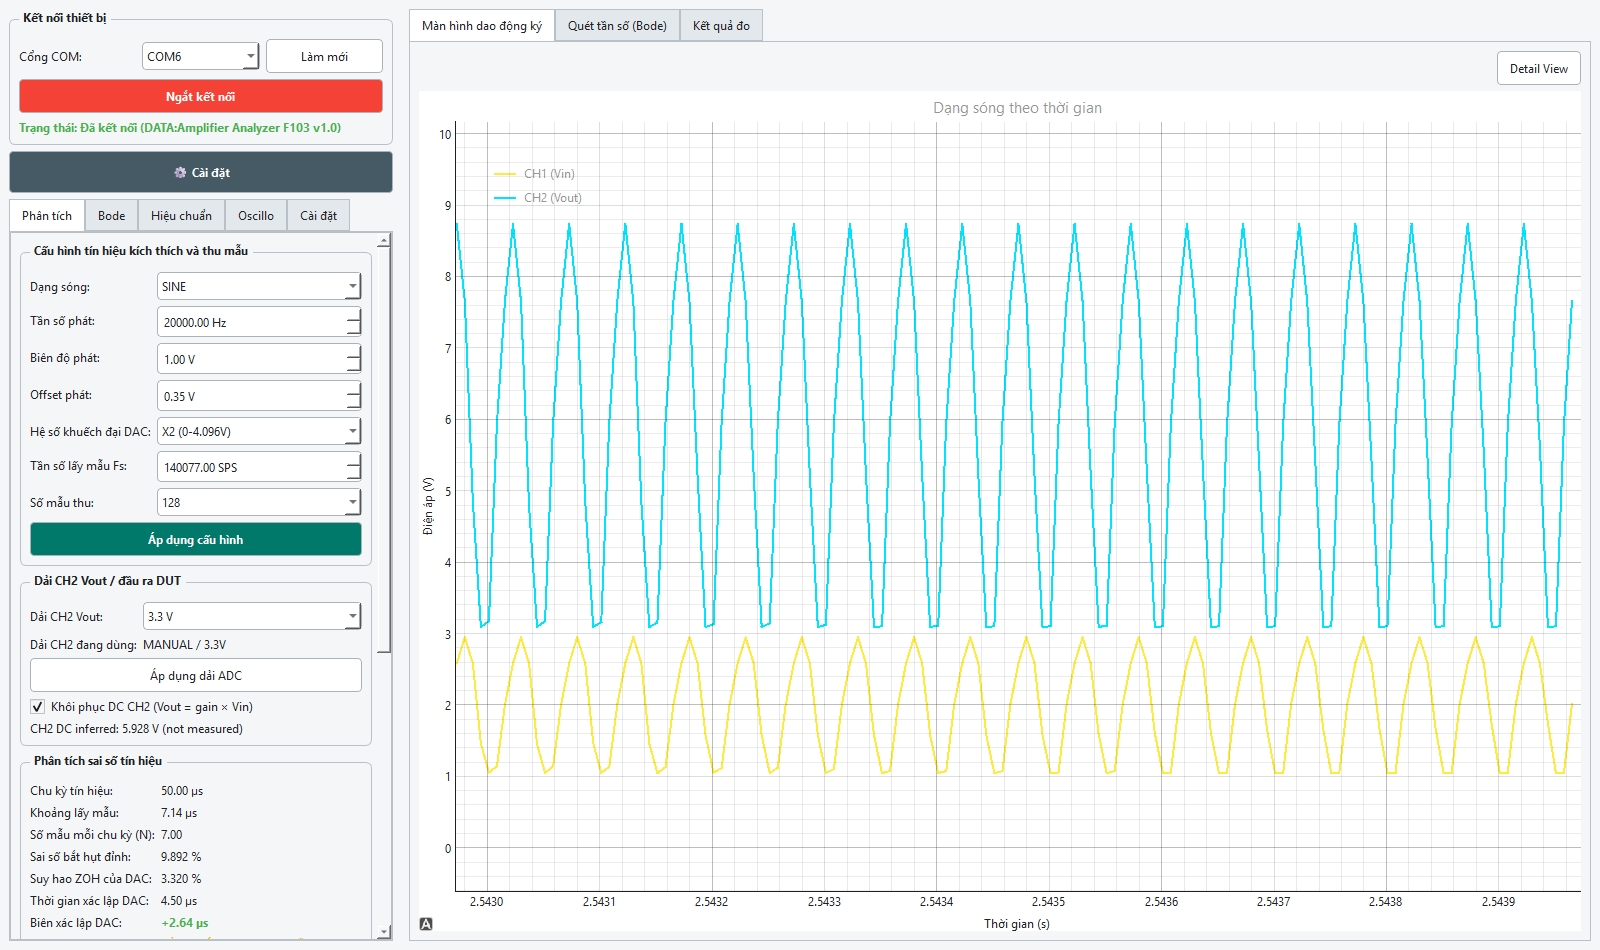
\includegraphics[width=0.82\textwidth]{images/result_app/05_freq_20000hz_waveform.png}\\[2mm]
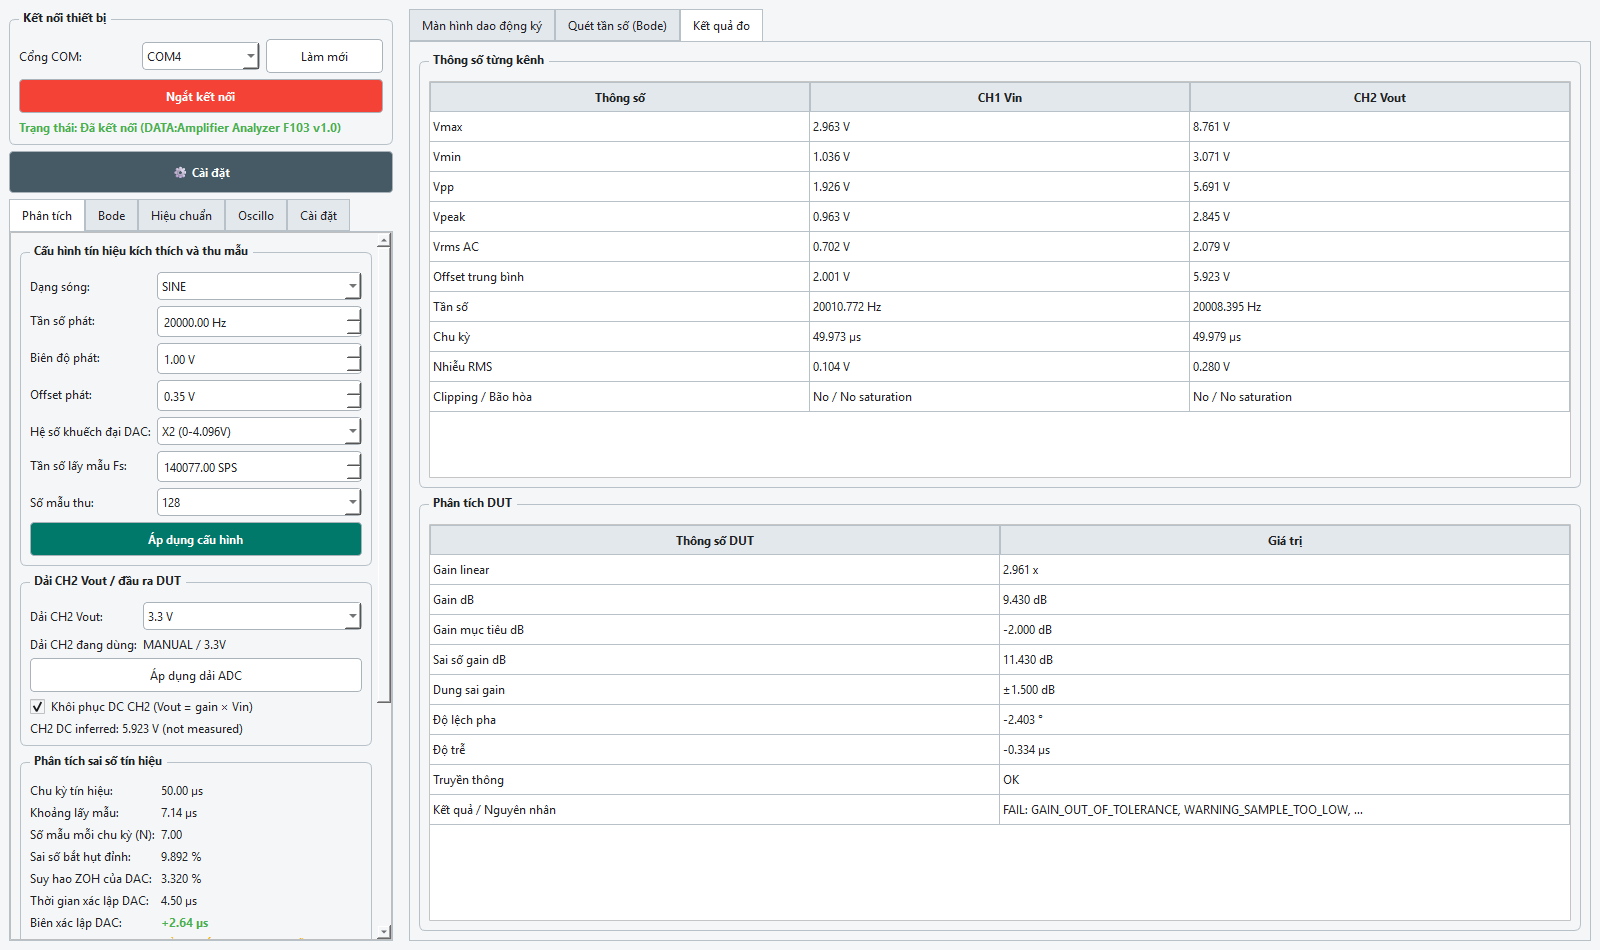
\includegraphics[width=0.82\textwidth]{images/result_app/05_freq_20000hz_results.png}
\caption{Kết quả thực tế tại $20\unit{kHz}$: waveform (trên) và bảng thông số (dưới)}
\label{fig:real_freq_20k}
\end{figure}

Ở $20\unit{kHz}$ chỉ còn xấp xỉ 7 mẫu mỗi chu kỳ. Hệ thống vẫn phát hiện được tần số cơ bản, song đường hiển thị có tính đa giác và sai số ước lượng đỉnh, pha hoặc méo tăng lên. Hình \ref{fig:real_freq_20k} vì vậy được đưa vào như một kết quả xấu có ý nghĩa: nó xác định trực tiếp giới hạn chất lượng của cấu hình hiện tại, dù điều kiện Nyquist vẫn được thỏa mãn.

\section{Kết quả thay đổi biên độ và dải đo}
\label{sec:real_range}
Ba ca dưới đây được chọn để minh họa ba cơ chế sai số khác nhau: clipping ở tín hiệu lớn, suy giảm tỷ số tín hiệu trên nhiễu ở tín hiệu rất nhỏ và bão hòa khi dải đo không phù hợp. Việc giữ lại các ca FAIL giúp đánh giá đúng nhược điểm của nguyên mẫu và vai trò của lựa chọn relay range.

\begin{figure}[H]
\centering
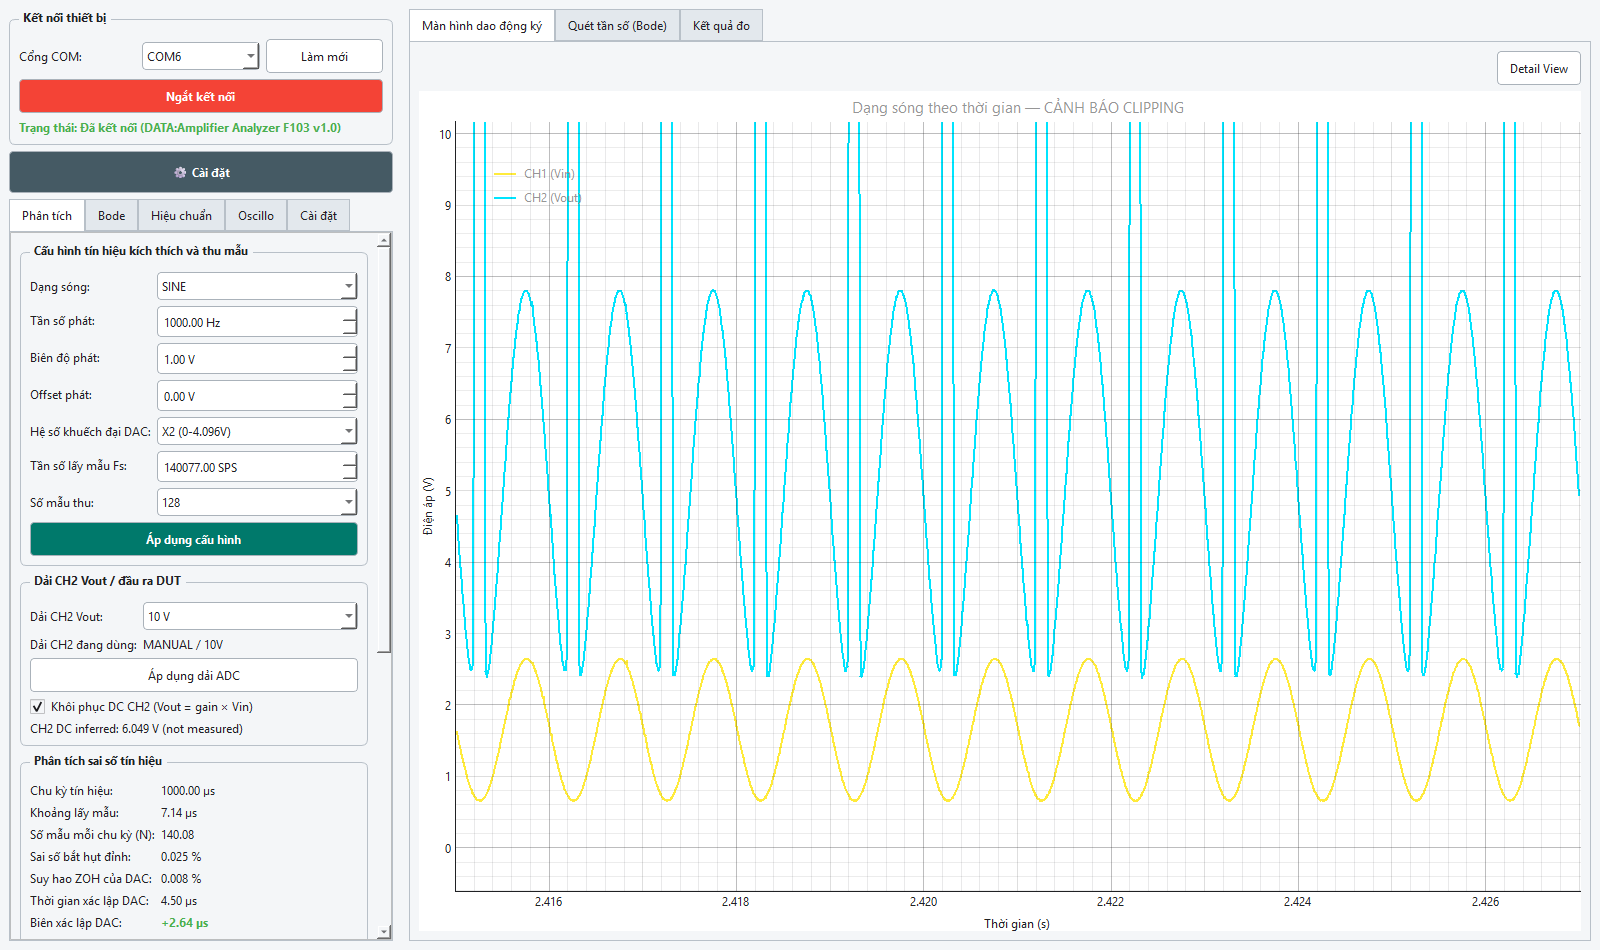
\includegraphics[width=0.82\textwidth]{images/result_app/06_amp_1p65_pm1_range10_waveform.png}\\[2mm]
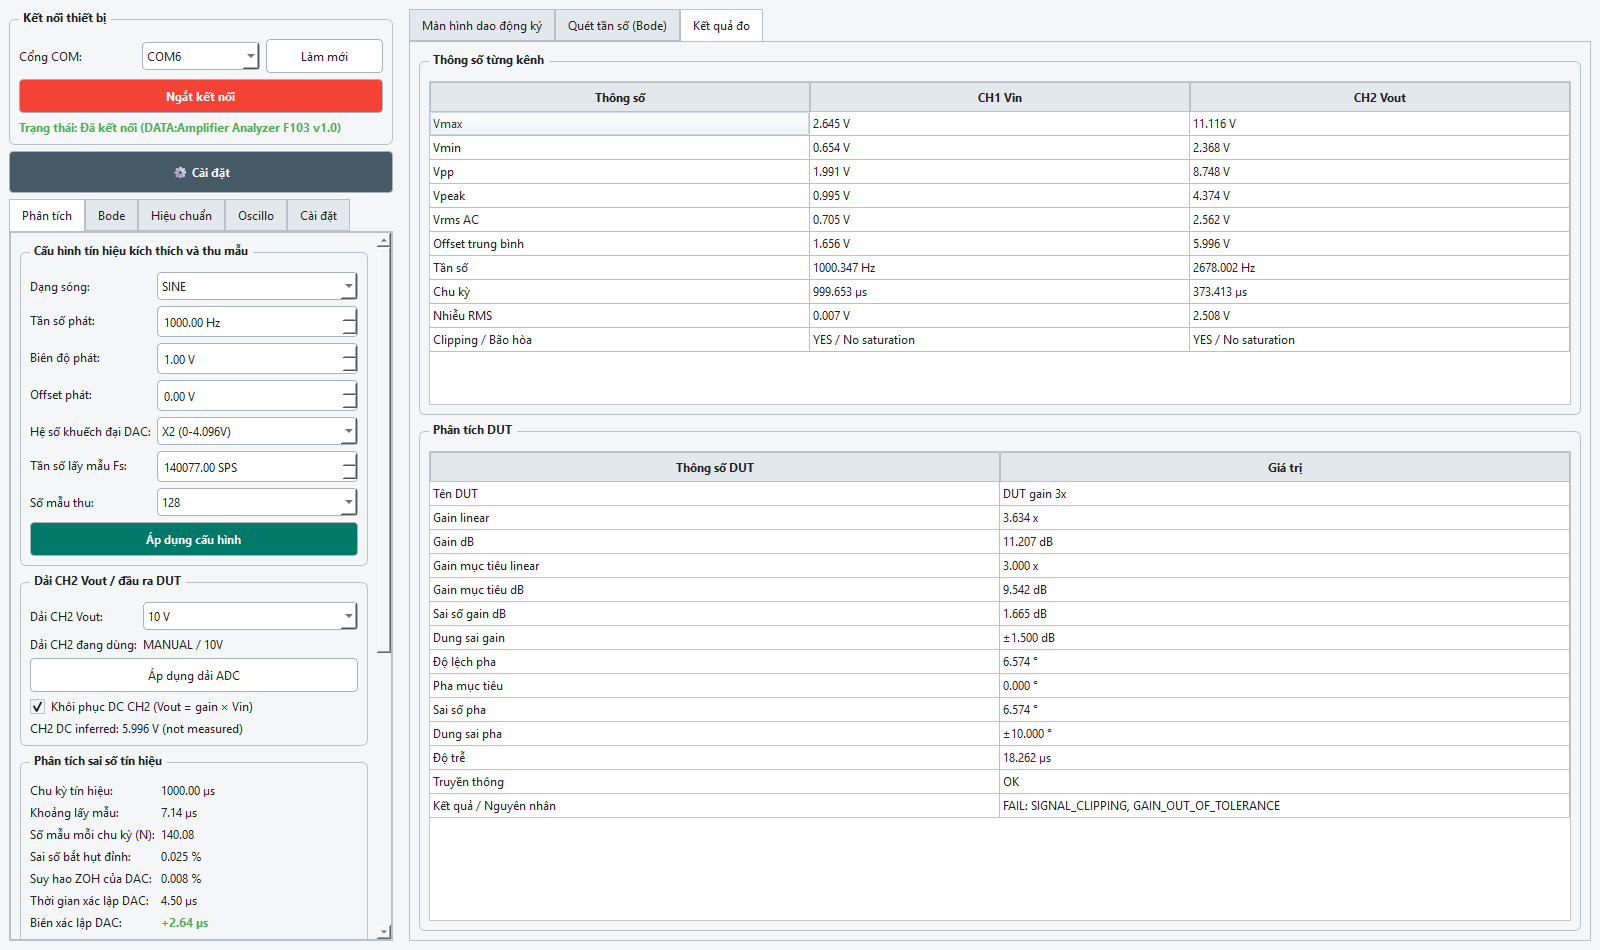
\includegraphics[width=0.82\textwidth]{images/result_app/06_amp_1p65_pm1_range10_results.png}
\caption{Tín hiệu $1{,}65\pm1\unit{V}$, dải $10\unit{V}$: phần waveform bị clipping và bảng kết quả FAIL}
\label{fig:real_range_10_large}
\end{figure}

Dải $10\unit{V}$ cho phép quan sát tín hiệu đầu ra lớn hơn, nhưng bản thân DUT/AFE vẫn có thể chạm giới hạn điện áp và làm bẹt đỉnh. Kết quả này cho thấy chọn dải rộng chỉ bảo vệ đầu vào ADC; nó không thể khắc phục clipping đã xuất hiện trước mạch chia áp. Thuật toán ước lượng tần số CH2 cũng bị ảnh hưởng khi waveform méo mạnh.

\begin{figure}[H]
\centering
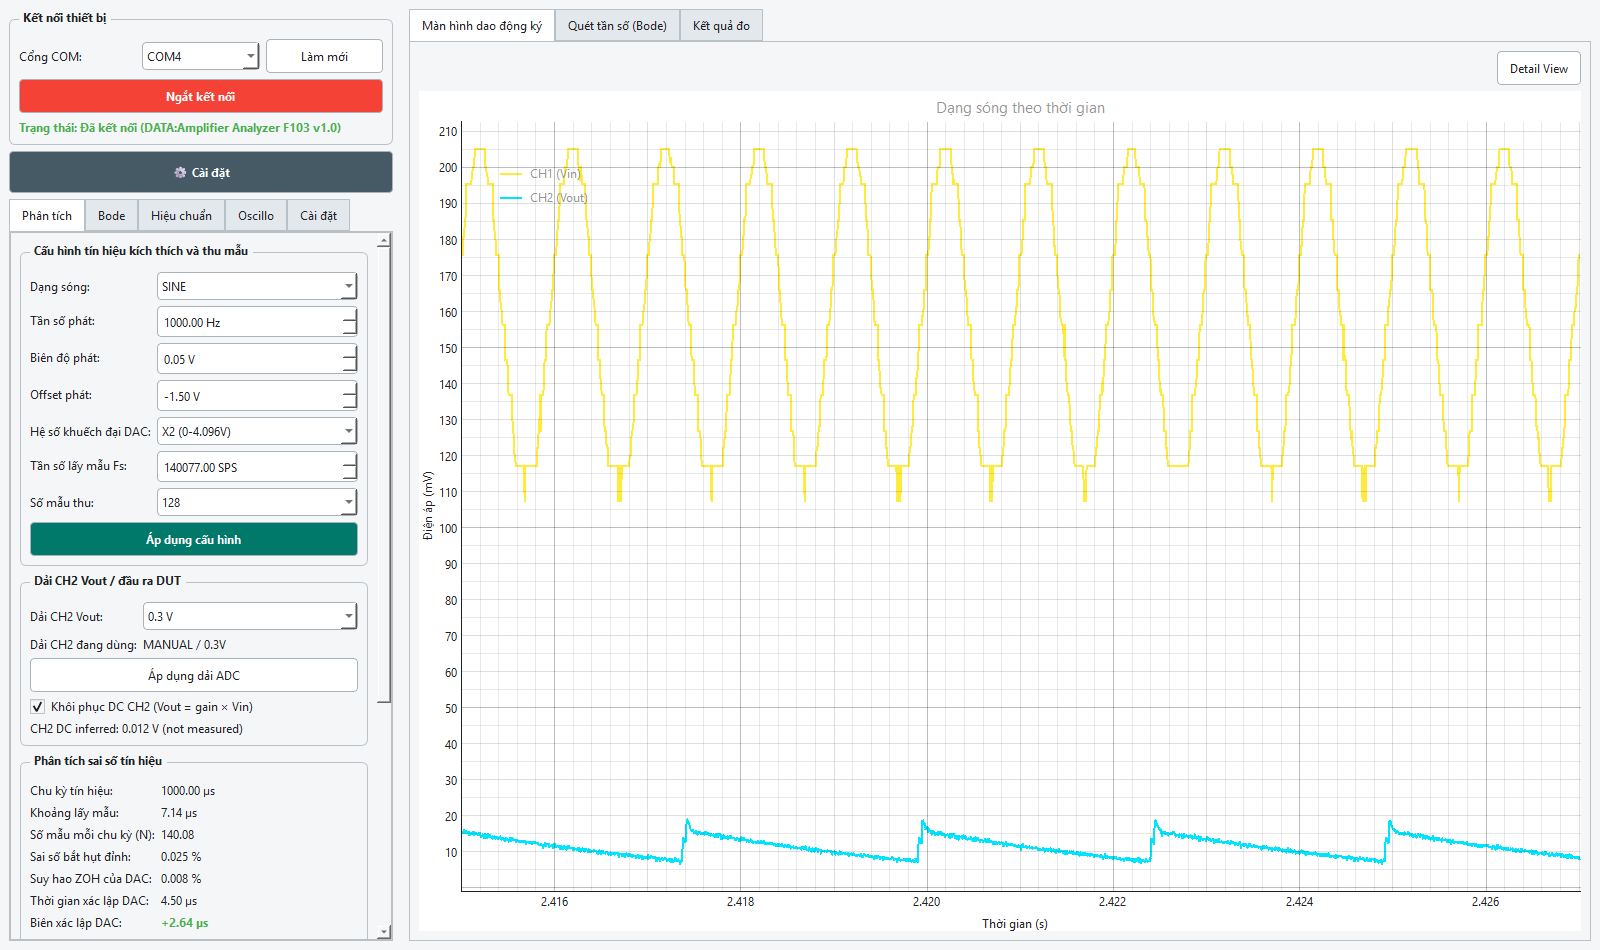
\includegraphics[width=0.82\textwidth]{images/result_app/08_amp_0p15_pm0p05_range0p3_waveform.png}\\[2mm]
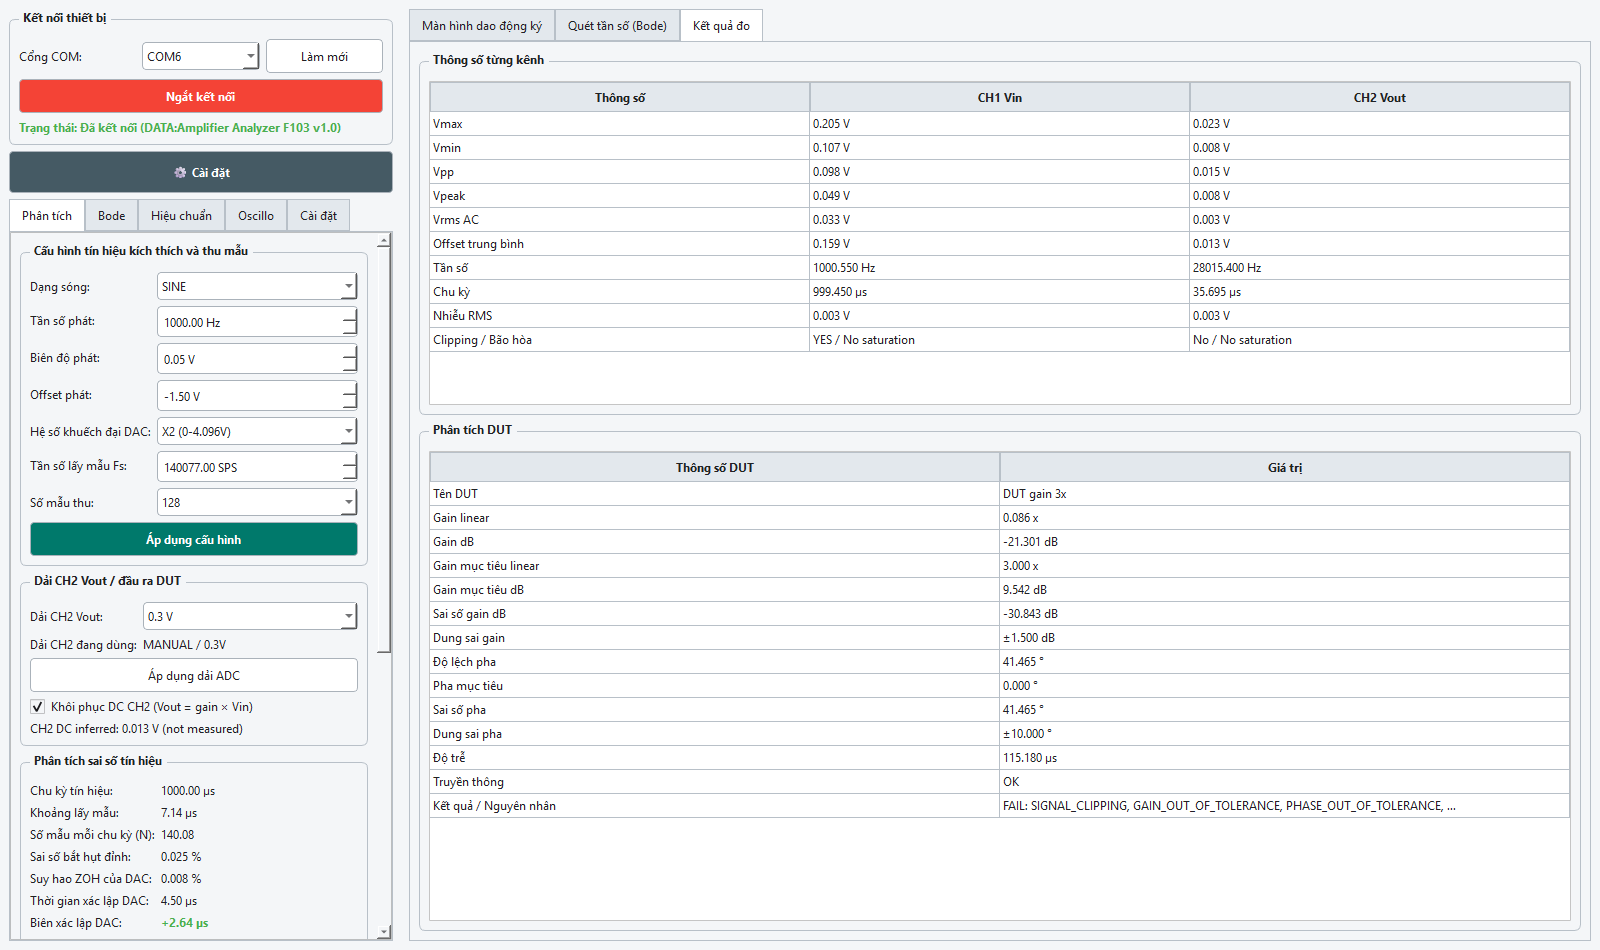
\includegraphics[width=0.82\textwidth]{images/result_app/08_amp_0p15_pm0p05_range0p3_results.png}
\caption{Tín hiệu nhỏ $0{,}15\pm0{,}05\unit{V}$, dải $0{,}3\unit{V}$: giới hạn tỷ số tín hiệu trên nhiễu}
\label{fig:real_range_03_small}
\end{figure}

Dải $0{,}3\unit{V}$ là lựa chọn đúng về nguyên tắc cho tín hiệu nhỏ, nhưng ảnh chụp thực tế cho thấy CH2 có biên độ gần nền nhiễu và thuật toán nhận dạng tần số không còn ổn định. Đây là trường hợp bất lợi của hệ thống: lượng tử hóa, nhiễu AFE và sai số offset chiếm tỷ lệ đáng kể so với tín hiệu cần đo.

\begin{figure}[H]
\centering
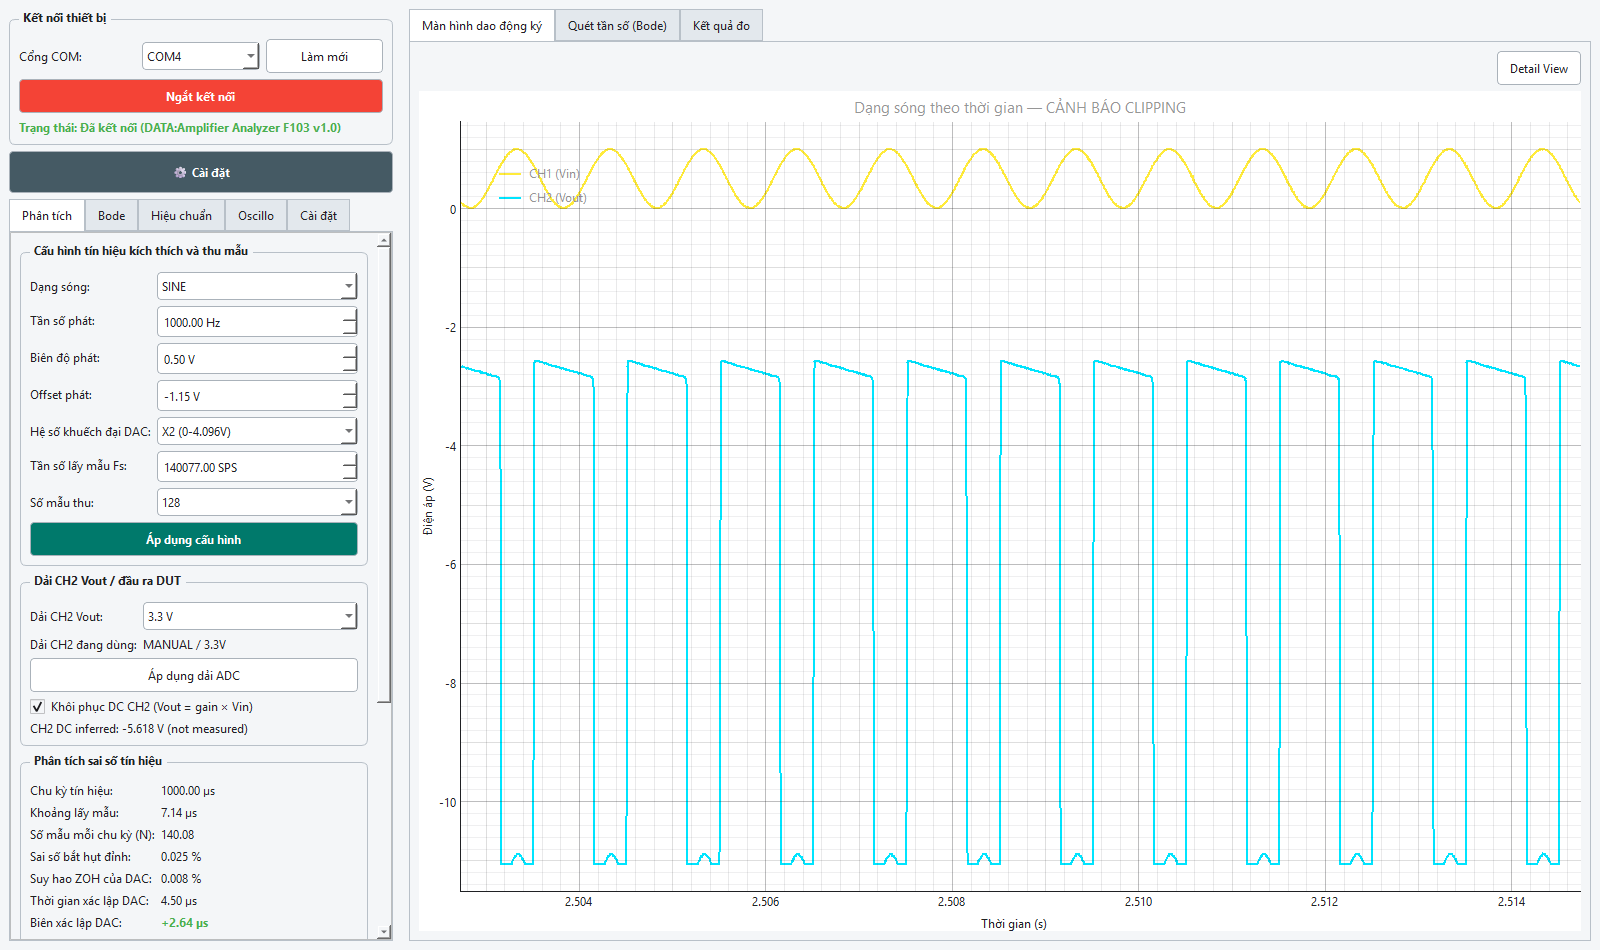
\includegraphics[width=0.82\textwidth]{images/result_app/09_amp_0p5_pm0p5_range3p3_waveform.png}\\[2mm]
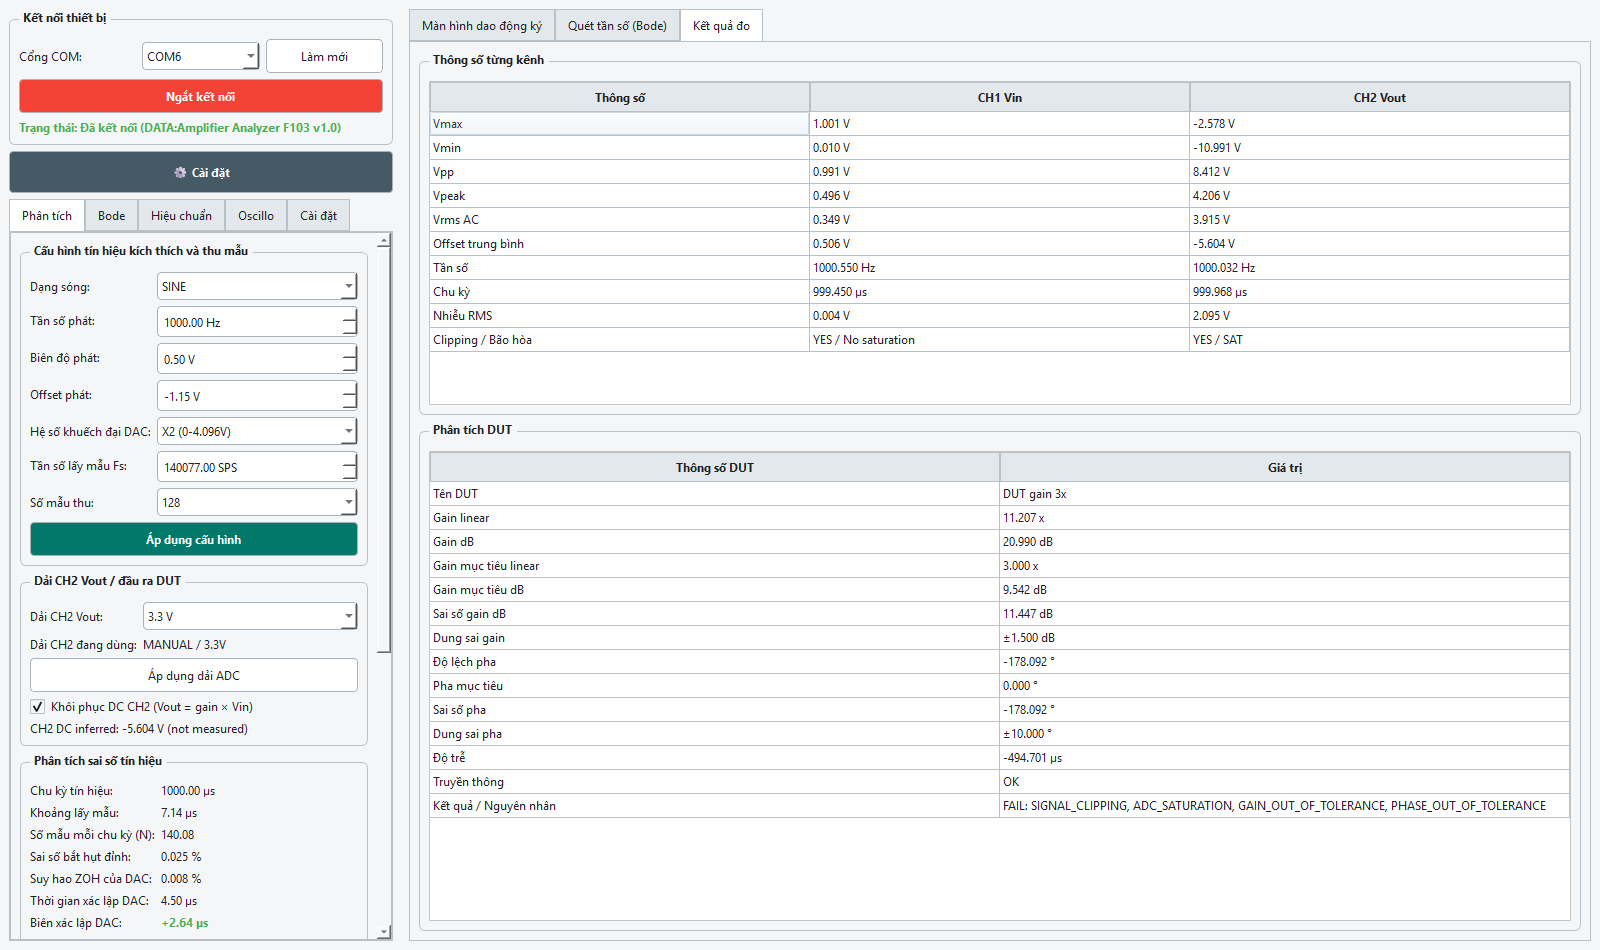
\includegraphics[width=0.82\textwidth]{images/result_app/09_amp_0p5_pm0p5_range3p3_results.png}
\caption{Tín hiệu $0{,}5\pm0{,}5\unit{V}$, dải $3{,}3\unit{V}$: bão hòa ADC và kết quả FAIL tương ứng}
\label{fig:real_range_33_sat}
\end{figure}

Ca dải $3{,}3\unit{V}$ thể hiện rõ trạng thái bão hòa và sai lệch lớn của CH2. Ứng dụng đã gắn cờ \code{ADC\_SATURATION}, \code{SIGNAL\_CLIPPING} và gain ngoài dung sai. Kết quả xác nhận cơ chế cảnh báo hoạt động, đồng thời cho thấy người dùng phải chọn dải theo điện áp đầu ra DUT chứ không suy ra từ biên độ do DAC phát.

\section{Kiểm nghiệm thuật toán đo}
Unit test sử dụng hai tín hiệu sine có offset khác nhau, gain 2 và phase $-30^\circ$. RMS AC loại đúng offset; gain linear thu được 2,000 và phase sai lệch dưới mức làm tròn của test. Test $20\unit{kHz}/200\unit{kSPS}$ xác nhận kết quả tổng thể là WARNING dù gain nằm trong tolerance.

Trong phép thử tích hợp với firmware SIM, kết quả đại diện ở Bảng \ref{tab:measurementresult} được tính từ dữ liệu mô phỏng. Bảng này xác nhận thuật toán và luồng USB SIM, không phải kết quả đo trên chuỗi analog thật.

\begin{table}[H]
\centering
\caption{Kết quả phân tích DUT chuẩn tại $20\unit{kHz}$}
\label{tab:measurementresult}
\begin{tabularx}{\textwidth}{|p{3.4cm}|p{3cm}|p{3.6cm}|X|}
\hline
\tableheadcolor\textbf{Thông số} & \textbf{Giá trị đặt} & \textbf{Giá trị đo} & \textbf{Nhận xét} \\ \hline
Tần số CH1 & $20.000\unit{Hz}$ & $19.999{,}4\unit{Hz}$ & Sai lệch nhỏ \\ \hline
Biên độ đỉnh Vin & $0{,}300\unit{V}$ & $0{,}300\unit{V}$ (sine fit) & Đạt \\ \hline
Gain linear & 0,800 & 0,800 & Đạt \\ \hline
Gain dB & $-1{,}938\unit{dB}$ & $-1{,}940\unit{dB}$ & Đạt \\ \hline
Phase & $-25{,}0^\circ$ & $-25{,}01^\circ$ & Đạt \\ \hline
Clipping/saturation & Không & Không & Đạt \\ \hline
Kết quả tổng & -- & WARNING & Do điều kiện lấy mẫu \\ \hline
\end{tabularx}
\end{table}

Trong simulation, Vpp đo trực tiếp khoảng $0{,}573\unit{V}$, nhỏ hơn $0{,}600\unit{V}$ lý tưởng do chỉ có 10 mẫu/chu kỳ. Trong khi đó sine fit khôi phục biên độ gần $0{,}300\unit{V}$. Kết quả này cho thấy lựa chọn RMS AC/sine fit phù hợp hơn max/min đối với dữ liệu sine mô phỏng ở cấu hình POC; hiệu quả trên phần cứng còn phụ thuộc sample timing thật.

\section{Kiểm nghiệm quét Bode}
Chế độ Bode mô phỏng quét theo dãy tần số logarithm. Với mô hình DUT có gain vùng thông xấp xỉ $-1{,}94\unit{dB}$ và đặc tính thông thấp bậc một, đường gain giữ ổn định trong vùng thông, giảm quanh tần số cắt và phase biến đổi liên tục. Worker quét chạy tách khỏi GUI nên thanh tiến độ và cửa sổ vẫn phản hồi.

Quét Bode trên phần cứng chưa được xác nhận. Source desktop hiện hard-code \code{SAMPLES=1024}, trong khi firmware production từ chối số mẫu lớn hơn 512; $F_s=10f$ cũng có thể vượt giới hạn tốc độ DAC/ADC. Khi lệnh hoặc JSON lỗi, worker hiện thay điểm bằng $-99\unit{dB}$ và $0^\circ$, vì vậy đồ thị phần cứng có thể chứa giá trị sentinel. Cần sửa cấu hình sweep, kiểm tra ACK từng lệnh và loại điểm lỗi rõ ràng trước khi công bố Bode đo thật.

\section{Phân tích sai số}
Các nguồn sai số chính gồm:
\begin{itemize}
    \item \textbf{Lượng tử ADC/DAC}: độ phân giải 12-bit tạo sai số tối thiểu theo LSB và tăng tương đối khi tín hiệu nhỏ.
    \item \textbf{Sampling phase}: max/min nhạy với vị trí mẫu, đặc biệt ở $N=10$.
    \item \textbf{DAC settling và ZOH}: hạn chế waveform ở tốc độ cập nhật cao.
    \item \textbf{AFE và range}: dung sai điện trở, offset op-amp và relay ảnh hưởng scale/offset.
    \item \textbf{Clock}: sai số thạch anh ảnh hưởng tần số phát, $F_s$ và phase.
    \item \textbf{Timing ADC}: tốc độ thực tế $140{,}077\unit{SPS}$ chỉ cung cấp khoảng 7 mẫu mỗi chu kỳ tại $20\unit{kHz}$, làm tăng độ nhạy của phép đo đỉnh và phase theo vị trí mẫu.
    \item \textbf{Framing và buffer}: pipeline SPI--DMA đã hoạt động liên tục, nhưng mất frame hoặc tràn buffer vẫn cần được giám sát bằng sequence number khi tăng tốc độ và thời gian stream.
    \item \textbf{Thuật toán}: zero crossing bị ảnh hưởng bởi nhiễu; sine fit giả định tín hiệu gần sine.
    \item \textbf{Truyền thông}: thiếu byte hoặc sai frame; được phát hiện bằng length và checksum.
\end{itemize}

Calibration tuyến tính bù được phần lớn sai số gain/offset tĩnh nhưng không bù hoàn toàn đặc tính theo tần số, jitter hoặc méo phi tuyến. Khi yêu cầu độ chính xác cao, cần calibration đa điểm theo tần số và biên độ.

\section{Thảo luận}
Ưu điểm của nguyên mẫu là kiến trúc đầy đủ từ phát, thu, truyền dữ liệu đến đánh giá chất lượng; có khả năng chạy không phần cứng; và tách được kiểm thử transport khỏi kiểm thử analog. Hai kênh ADC đồng thời về nguyên lý phù hợp với phép đo phase. Giao thức request/response dễ debug, trong khi frame nhị phân giảm overhead khi truyền mẫu.

Kết quả phần cứng thật cho thấy chuỗi analog và timing thu đã hoạt động, nhưng chất lượng chưa đồng đều trên toàn miền đo. Ở tần số thấp, waveform trơn và quan hệ khuếch đại giữa hai kênh quan sát được rõ. Ngược lại, tại $20\unit{kHz}$ chỉ còn 7 mẫu/chu kỳ; tín hiệu rất nhỏ bị chi phối bởi nhiễu và offset; tín hiệu lớn có thể clipping trước ADC; lựa chọn dải chưa phù hợp gây bão hòa. Các ảnh FAIL được giữ lại để phản ánh đúng các giới hạn này. Ngoài ra, checksum XOR chỉ phát hiện lỗi đơn giản và phép sine fit không phù hợp với waveform đã méo mạnh; các trường hợp đó cần FFT hoặc bộ ước lượng có kiểm tra độ phù hợp mô hình.

\chapter{KẾT LUẬN VÀ HƯỚNG PHÁT TRIỂN}

\section{Kết luận}
Đồ án đã xây dựng được nguyên mẫu hệ thống phân tích tín hiệu khuếch đại gồm phần cứng STM32F103C8T6, MCP4822, ADS7861, mạch lựa chọn range, firmware USB CDC và ứng dụng Signal Analyzer Pro. Phần USB/protocol, DAC DMA, ADC timer--SPI--DMA, stream liên tục và pipeline phân tích trên desktop đã hoạt động. Chuỗi analog từ DAC qua DUT/AFE tới ADS7861 đã được xác nhận end-to-end bằng chín cấu hình đo thật và ảnh chụp ứng dụng. Kết quả đủ để đánh giá chức năng nguyên mẫu, nhưng chưa thay thế phép hiệu chuẩn với thiết bị chuẩn để công bố độ chính xác gain, phase hoặc Bode.

Điểm khác biệt quan trọng là kết quả được đánh giá cùng điều kiện đo. Tốc độ ADC thực tế $140{,}077\unit{SPS}$ tạo khoảng 1401 mẫu/chu kỳ ở $100\unit{Hz}$, 28 mẫu/chu kỳ ở $5\unit{kHz}$ và 7 mẫu/chu kỳ ở $20\unit{kHz}$. RMS AC và sine fit giúp giảm ảnh hưởng bỏ lỡ đỉnh khi waveform còn gần sine, nhưng không khắc phục được clipping, bão hòa hoặc tỷ số tín hiệu trên nhiễu thấp. Vì vậy báo cáo trình bày đồng thời trường hợp tốt và xấu, thay vì chỉ dùng các ảnh có dạng sóng thuận lợi.

\section{Đánh giá mức độ hoàn thành}
Các mục tiêu về giao tiếp USB, điều khiển DAC, format dữ liệu hai kênh, stream liên tục, DSP, PASS/FAIL/WARNING, calibration và export đã được triển khai. Firmware production đã build, nạp và chạy trên STM32F103C8T6. Ứng dụng dùng tiến trình đọc riêng để tránh khóa giao diện; bộ chụp báo cáo gồm chín cấu hình phần cứng thật, mỗi cấu hình có waveform, bảng kết quả và metadata truy vết. Trong toàn bộ đợt chụp, giao tiếp COM4 được ghi nhận hoạt động và tốc độ lấy mẫu hiển thị ổn định ở $140{,}077\unit{SPS}$.

\section{Hạn chế của hệ thống}
ADC hiện đạt khoảng $140\unit{kSPS}$, tương đương 7 mẫu/chu kỳ tại $20\unit{kHz}$; mức này đủ phát hiện tần số nhưng còn thấp cho đánh giá chi tiết waveform và phase. DAC stream có thể chạy $200\unit{kSPS}$ nhưng khoảng cập nhật $5\unit{\mu s}$ sát settling time. Auto-range dùng relay có thời gian chuyển mạch lớn hơn switch bán dẫn và người dùng vẫn phải chọn dải theo đầu ra DUT. Phép đo DC của CH2 trên ứng dụng còn có thành phần suy ra theo mô hình thay vì đo trực tiếp. Calibration Flash chưa có magic/version/CRC; checksum XOR của frame yếu hơn CRC-16/CRC-32. Phép đo noise/phase hiện tối ưu cho sine và chưa thay thế thiết bị đo chuẩn.

\section{Hướng phát triển}
\subsection{Nâng cấp nền tảng xử lý để hướng tới sai số 1\% tại 20 kHz}
Với cấu hình hiện tại, $F_s=140{,}077\unit{SPS}$ chỉ tạo khoảng 7 mẫu mỗi chu kỳ ở $20\unit{kHz}$. Nếu chỉ xét sai số bỏ lỡ đỉnh trong trường hợp bất lợi, điều kiện
\begin{equation}
1-\cos\left(\frac{\pi}{N}\right)<1\%
\end{equation}
yêu cầu xấp xỉ $N\geq23$ mẫu/chu kỳ, tức $F_s\geq460\unit{kSPS}$. Do đó mục tiêu thực tế nên là tối thiểu $500\unit{kSPS}$ cho hai kênh đồng thời, kết hợp sine fit/FFT, clock ổn định và hiệu chuẩn toàn chuỗi. ADS7861 hiện tại có giới hạn danh định $500\unit{kSPS}$ nên chính ADC cũng đã ở sát ngưỡng cần thiết; nếu cần thêm biên dự phòng phải thay bằng ADC nhanh hơn.

Bảng \ref{tab:mcu_upgrade} so sánh ba lựa chọn MCU phổ biến. STM32F411CE là bước nâng cấp vừa phải về Flash/RAM nhưng mức tăng CPU và USB chưa tạo nhiều dư địa cho đồng thời lấy mẫu tốc độ cao, đóng gói frame, kiểm tra lỗi, DSP và cập nhật giao diện. STM32H743ZI phù hợp hơn cho phiên bản tiếp theo nhờ Cortex-M7 đến $480\unit{MHz}$, cache, DMA mạnh, SRAM lớn và USB High Speed \cite{stm32f411ds,stm32h743ds}.

\begin{table}[H]
\centering
\caption{So sánh nền tảng MCU cho hướng nâng cấp}
\label{tab:mcu_upgrade}
\footnotesize
\begin{tabularx}{\textwidth}{|p{2.25cm}|p{2.7cm}|p{1.45cm}|p{1.35cm}|p{2.1cm}|p{1.35cm}|X|}
\hline
\tableheadcolor\textbf{MCU} & \textbf{CPU} & \textbf{Flash} & \textbf{RAM} & \textbf{USB} & \textbf{UART} & \textbf{Đánh giá} \\ \hline
STM32F103C8 & Cortex-M3, $72\unit{MHz}$ & $64\unit{kB}$ & $20\unit{kB}$ & USB FS Device & 3 & Đủ cho nguyên mẫu hiện tại. \\ \hline
STM32F411CE & Cortex-M4, $100\unit{MHz}$ & $512\unit{kB}$ & $128\unit{kB}$ & USB OTG FS & 3 & Nâng cấp kinh tế, dư địa vừa phải. \\ \hline
STM32H743ZI & Cortex-M7, $480\unit{MHz}$ & $2\unit{MB}$ & đến $1\unit{MB}$ & USB OTG FS+HS & 8+ & Phù hợp cho phiên bản đo tốc độ cao. \\ \hline
\end{tabularx}
\end{table}

STM32H743ZI giải quyết trực tiếp ba nút thắt phần mềm: (i) đủ năng lực duy trì SPI/DMA hai kênh ở khoảng $500\unit{kSPS}$ trong khi chạy DSP; (ii) đủ RAM cho ping-pong/ring buffer lớn, chấp nhận độ trễ truyền lên ứng dụng mà không mất mẫu; và (iii) USB HS tạo biên thông lượng lớn hơn USB FS. Tuy nhiên, thay MCU không tự động bảo đảm sai số 1\%. Để công bố đạt spec, thiết kế mới còn phải dùng ADC/DAC có tốc độ và settling phù hợp, AFE đủ băng thông và tuyến tính, clock có jitter thấp, layout tốt, hiệu chuẩn đa điểm và kiểm chứng bằng máy phát/oscilloscope chuẩn. Vì vậy STM32H7 là điều kiện tạo dư địa xử lý cần thiết, không phải điều kiện duy nhất.

Các hướng phát triển kỹ thuật tiếp theo gồm:
\begin{itemize}
    \item Chuyển pipeline DMA hiện tại sang ping-pong/ring buffer nhiều khối và gắn sequence number để chứng minh không mất mẫu trong phép đo dài.
    \item Dùng một timebase chính xác chung cho DAC và ADC; trả về sample rate đo được và thống kê jitter.
    \item Xác minh BUSY, 32 clock, cạnh lấy mẫu, status A/B và thứ tự word ADS7861 bằng logic analyzer ở tốc độ cực đại.
    \item Đo đồng thời MCP4822 VOUTA, các chân vi sai ADS7861, reference và nguồn AFE để xây dựng ngân sách sai số end-to-end.
    \item Sửa Bode sweep theo giới hạn 128/256/512 mẫu, kiểm ACK từng điểm và không vẽ sentinel như dữ liệu hợp lệ.
    \item Sử dụng DAC có settling nhanh hơn hoặc DDS chuyên dụng khi đo tần số cao.
    \item Bổ sung trigger oscilloscope, FFT, THD, SNR, SINAD và group delay.
    \item Nâng checksum lên CRC-16/CRC-32 và thêm sequence number để phát hiện mất frame.
    \item Calibration đa điểm theo range, tần số và biên độ; lưu hồ sơ truy xuất chuẩn.
    \item Thiết kế phiên bản STM32H743ZI, ưu tiên SPI/DMA, cache coherency, USB HS và buffer SRAM lớn cho streaming liên tục.
    \item Hoàn thiện vỏ thiết bị, connector BNC, bảo vệ đầu vào và quy trình tự kiểm tra.
\end{itemize}

% ==================== TÀI LIỆU THAM KHẢO ====================
\addcontentsline{toc}{chapter}{TÀI LIỆU THAM KHẢO}
\begin{thebibliography}{99}
\bibitem{stm32ds} STMicroelectronics, \textit{STM32F103x8, STM32F103xB Medium-density Performance Line ARM-based 32-bit MCU Datasheet}, DS5319, STMicroelectronics.
\bibitem{stm32rm} STMicroelectronics, \textit{RM0008: STM32F101xx, STM32F102xx, STM32F103xx, STM32F105xx and STM32F107xx Reference Manual}.
\bibitem{stm32f411ds} STMicroelectronics, \textit{STM32F411xC/E Arm Cortex-M4 32-bit MCU Datasheet}, DS10314, STMicroelectronics.
\bibitem{stm32h743ds} STMicroelectronics, \textit{STM32H742xI/G, STM32H743xI/G Arm Cortex-M7 32-bit MCU Datasheet}, DS12110, STMicroelectronics.
\bibitem{mcp4822} Microchip Technology Inc., \textit{MCP4802/4812/4822: 8/10/12-Bit Dual Voltage Output Digital-to-Analog Converter with Internal VREF and SPI Interface}, Datasheet DS20002249.
\bibitem{ads7861} Texas Instruments, \textit{ADS7861: Dual, 500-kSPS, 12-Bit, 2+2 Channel, Simultaneous Sampling Analog-to-Digital Converter}, Datasheet SBAS110.
\bibitem{usbcdc} USB Implementers Forum, \textit{Universal Serial Bus Class Definitions for Communications Devices}, Revision 1.2.
\bibitem{oppenheim} A. V. Oppenheim and R. W. Schafer, \textit{Discrete-Time Signal Processing}, 3rd ed. Pearson, 2010.
\bibitem{numpy} NumPy Developers, \textit{NumPy Documentation}. [Online]. Available: \url{https://numpy.org/doc/}
\bibitem{scipy} SciPy Community, \textit{SciPy Documentation}. [Online]. Available: \url{https://docs.scipy.org/doc/scipy/}
\bibitem{pyqt} Riverbank Computing, \textit{PyQt6 Reference Guide}. [Online]. Available: \url{https://www.riverbankcomputing.com/static/Docs/PyQt6/}
\bibitem{pyqtgraph} PyQtGraph Developers, \textit{PyQtGraph Documentation}. [Online]. Available: \url{https://pyqtgraph.readthedocs.io/}
\bibitem{pyserial} C. Liechti, \textit{pySerial Documentation}. [Online]. Available: \url{https://pyserial.readthedocs.io/}
\end{thebibliography}

\end{document}
